\chapter{\ifproject%
\ifcpe การทดลองและผลลัพธ์\else Experimentation and Results\fi
\else%
\ifcpe การทดลองและผลลัพธ์\else System Evaluation\fi
\fi}
\quad ในบทนี้จะกล่าวถึงการนำ prototype ไปทดสอบกับกลุ่มผู้ใช้งาน (potential user) โดยจะเป็นการให้โจทย์กับผู้ทดสอบแล้วปล่อยให้ใช้งาน prototype โดยใช้ความรู้สึก และ ความเคยชินของผู้ทดสอบเอง 
เพื่อที่จะวัดว่าระบบของเรามีความสอดคล้องกับ ux ของผู้ทดสอบเพียงใดและต้องปรับปรุงตรงไหนบ้าง โดยโจทย์ที่ให้กับผู้ทดสอบมีดังนี้ \ref{fig:eval_test}

\section{สร้างบริษัทของคุณ} 
ในขั้นตอนนี้ผู้ทดสอบจะต้องทำการกดปุ่มสร้างบริษัทใหม่ในหน้าแรก ดังรูป \ref{fig:index} จากนั้นระบบก็จะแสดงวิธีการสร้างบริษัทใหม่ดังรูป \ref{fig:create_company}
และ หากทำตามขั้นตอนที่เขี่ยนไว้ในวิธีการ คือ 1. เพิ่มเพื่อนกับ PenHwang โดยใช้การสแกน qr code หรือ ค้นหาชื่อ 2. พิมพ์คำว่า "สร้างบริษัทใหม่" 3. นำรหัสที่ตอบกลับมาไปใส่ในช่องที่กำหนด
ก็จะไปถึงหน้าตั้งค่าบริษัท ดังรูป \ref{fig:setting} จากนั้นทำการกรอกข้อมูลเบื้องต้นของบริษัทประกอบด้วย ชื่อ คำบรรยาย email เบอร์โทรศัพท์ และ ที่อยู่ของบริษัท

เนื่องจากผู้พัฒนาคิดว่าคนที่สร้างบริษัทก็จะเป็นพนักงานคนนึง จึงได้สร้างพนักงานโดยใช้ LINE id ของคนที่สร้างบริษัท ขั้นตอนต่อไปจึงเป็นการกรอกข้อมูลส่วนตัวของผู้สร้างบริษัท 
โดยการไปที่หน้าผู้จัดการ ดังรูป \ref{fig:manager} จากนั้นก็กรอกข้อมูลส่วนตัวของตนเองลงไปเป็นอันเสร็จขั้นตอนการสร้างบริษัท

ในขั้นแรกผู้ทดสอบสามารถทำได้แบบไม่ติดขัดอะไรนั้นแสดงว่า ux ณ จุดนี้ดีอยู่แล้ว แต่ผู้ทดสอบทำได้ราบรื่นจนถึงขั้นตอนการตั้งค่าเท่านั้น การกรอกข้อมูลส่วนตัวของตนเองนั้นยังต้องมีการบอกให้ทำ
นั้นแสดงว่า ต้องเพิ่มการสอนการเพิ่มผู้สร้างบริษัทเข้าสู่บริษัทด้วย และ มีคำแนะนำจากผู้ทดสอบว่าปุ่มลบบริษัทเด่นนั้นจนเกินไป และ ตอนสร้างบริษัทไม่ควรมีปุ่มนี้อยู่

\section{เพิ่มพนักงานอีก 1 คนเข้าสู่บริษัท}
ในขั้นตอนนี้ผู้ทดสอบต้องให้พนักงานอีกคนเพิ่มเพื่อนกับ PenHwang จากนั้นพิมพ์คำว่า "ฉันเป็นพนักงานใหม่" จะมี button message ตอบกลับมา ดังรูป \ref{fig:message_start_form}
เมื่อคลิ๊กเข้าไปแล้วจะเป็นแบบฟอร์มการเริ่มต้นเป็นพนังงานให้กรอกข้อมูลซี้งประกอบด้วย รหัสสำหรับบริษัท (passcode) ซึ่งได้จากหน้าตั้งค่าบริษัท \ref{fig:setting} และ ข้อมูลส่วนตัว เช่น ชื่อ เบอร์ติดต่อ email และ LINE id ดังรูป \ref{fig:line_start_form} 
จากนั้นหากกดส่ง 
ก็จะเป็นการส่งคำขอเข้าร่วมบริษัทไปที่บริษัทนั้น จากนั้นพนักงานฝ่ายบุคคลก็จะเป็นคนรับคำขอที่หน้า dashboard ดังรูป \ref{fig:dashboard} หรือ หน้าพนักงาน ดังรูป \ref{fig:new_employee}

ในขั้นตอนนี้ทางผู้พัฒนาไม่ได้ใส่จุดที่สอนวิธีการเพิ่มพนักงานเพราะผู้พัฒนาคิดว่าขั้นตอนการเพิ่มพนักงานอีก เหมือนกับการเพิ่มผู้สร้างบริษัททุกประการ แต่เมื่อทำการทดสอบแล้ว 
พบว่าผู้ทำการทดสอบไม่รู้ว่าต้องเพิ่มพนักงานอย่างไรทำให้ต้องบอกเป็นขั้นตอนเพื่อให้ไปถึงขั้นต่อไปได้

\section{สร้างตารางงานให้พนักงานคนนั้น}
ในขั้นตอนนี้ผู้ทดสอบต้องเข้าไปที่หน้า ตารางงานหรือกะ \ref{fig:slot} จะพบว่ามีกะที่สร้างไว้อยู่แล้วชื่อ default slot ซึ่งเป็นกะที่เริ่มงาน 9.30 น. ออกงาน 17.30 น. ทุกวันยกเว้นวันอาทิตย์ที่ไม่ทำงาน 
ผู้พัฒนาทำการใส่เอาไว้เพื่อเป็นตัวอย่างการจัดตารางงานให้พนักงาน หรือ หากบริษัทใดมีการทำงานที่ใกล้เคียงกันก็สามารถเปลี่ยนการตั้งค่าเล็กน้อยแล้วใช้งานตารางนี้ได้ แต่ในขั้นตอนี้ผู้ทดสอบจะต้องไปที่หน้า 
สร้างตารางใหม่ จากนั้นก็จะมีตารางให้เริ่มกรอกข้อมูลซึ่งประกอบด้วย ชื่อตาราง สายหลังจากผ่านไป เวลาเข้า-ออกงานของแต่ละวัน และ พนักงานที่จะให้ใช้ตารางนี้ ดังรูป \ref{fig:new_slot} 
จากนั้นมื่อเพิ่มพนักงานเข้าสู่กะแล้วก็จะมีข้อความส่งไปที่พนักงานคนนั้นด้วย ดังรูป \ref{fig:added_slot}

ในขั้นตอนนี้ผู้ทดสอบมีความสับสนเล็กน้อยกับข้อความในหน้าสร้างตารางใหม่ คือ คำว่า "สายหลังจาก" ซึ่งความหมายของมันคือสายหลังจากผ่านไปกี่นาที แต่ผู้ทดสอบสับสนว่าเป็นสายหลังจากเวลาเท่าใด

\section{ให้พนักงานดูตารางเวลาทำงานของตนเอง}
ในขั้นตอนนี้ผู้ทดสอบต้องทำการกด rich menu ปุ่มดูตารางงานของฉันใน LINE ดังรูป \ref{fig:rich_menu} จากนั้นจะได้รับข้อความตอบกลับในรูแบบ flex message ที่บอกเวลาที่ต้องเข้า-ออกงานในแต่ละวัน ดังรูป \ref{fig:message_slot}

\section{สร้างจุดลงเวลา}
ในขั้นตอนนี้ผู้ทดสอบต้องไปที่หน้า จุดลงเวลา \ref{fig:location} และกดที่ปุ่มสร้างจุดลงเวลาใหม่ \ref{fig:new_location} จากนั้นก็กรอกข้อมูลซึ่งประกอบด้วย ชื่อจุดลงเวลา ระยะที่สามารถห่างได้ 
ผู้พัฒนาได้จำกัดระยะนี้ไว้น้อยสุดที่ 50 เมตรเพื่อป้องกัน ความผิดพลาดจากการเช็คตำแหน่งที่อยู่ จุดลงเวลาโดยใช้ Google map API มาแสดงและเก็บค่า และ พนักงานที่จะใช้จุดลงเวลานี้ 
จากนั้นมื่อเพิ่มพนักงานเข้าสู่กะแล้วก็จะมีข้อความส่งไปที่พนักงานคนนั้นด้วย \ref{fig:added_location}

\section{เช็คชื่อเข้า-ออกงาน}
ในขั้นตอนนี้ผู้ทดสอบต้องทำการกด rich menu ปุ่มขอลงเวลาใน LINE ดังรูป \ref{fig:rich_menu} จากนั้นจะได้รับข้อความตอบกลับในรูแบบ button message โดยหากไม่ได้เข้างานอยู่
จะเป็นข้อความเพื่อเข้างาน แต่ หากเข้างานอยู่แล้วข้อความที่ส่งมาก็จะเปลี่ยนเป็นข้อความเพื่อออกงาน ดังรูป \ref{fig:clock_in} และ \ref{fig:clock_out} เมื่อกด button message เข้าไปจะเป็น 
web applicaion ที่แสดงว่าสามารถเข้า หรือออกงานตรงนี้ได้หรือไม่ หาไม่ได้จะมีข้อความแสดงผลดังรูป \ref{fig:cant_clock} 
แต่หากสามารถเข้างานได้จะแสดงปุ่มเพื่อเข้า หรือออกงาน ดังรูป \ref{fig:clock} 
จากนั้นหากต้องการดูประวัตการเข้าออกงานของพนักงานสามารถเข้าไปดูได้ที่หน้าพนักงาน/เลือกพนักงานคนนั้น/ประวัติการทำงาน ดังรูป \ref{fig:history} โดยจะแสดงวันเวลาที่เข้า-ออก ลา หรือ ขาดงาน
ละเมื่อคลิ๊กที่การเข้าหรือออกงาน ก็จะเป็นการแสดงสถานที่ที่พนักงานคนนั้นเข้าหรือออกงานได้ด้วย
หรือ สามารถดูสรุปประวัติการทำงานของพนักงานทุกคนได้ที่หน้าเงินเดือน 
ส่วนพนักงานเองก็สามารถดูประวัติการเข้าออกงานของตนเองได้เหมือนกันโดยคลิ๊ก rich menu ปุ่มตั้งค่า จากนั้นจะได้รับข้อความตอบกลับในรูแบบ carousel button message 
ดังรูป \ref{fig:message_setting}
จากนั้นเลือก ข้อมูลส่วนตัว จะเป็นการเข้าสู่เว็บแอปพลิเคชันที่แสดงข้อมูลของพนักงานประกอบด้วย ข้อมูลส่วนตัว ประวัติการทำงาน และ สิทธิการลา ดังรูป \ref{fig:line_personal_info}

\section{สร้างประเภทการลา}
ในขั้นตอนนี้ผู้ทดสอบต้องเข้าไปที่หน้า \ref{fig:leave} ประเภทการลาและกดปุ่มสร้างประเภทใหม่ \ref{fig:new_leave} 
จากนั้นก็กรอกข้อมูลซึ่งประกอบด้วย ชื่อประเภทการลา สิทธิ์การลา และพนักงานที่สามารถใช้การลานี้ได้
และเมื่อเพิ่มพนักงานให้สามารถใช้ประเภทการลานั้น ๆ ได้ก็จะส่งข้อความไปหาพนักงานด้วยดังรูป \ref{fig:added_leave}

โดยในขั้นตอนการขอดูตารางเวลาทำงานขอตนเอง เช็คชื่อเข้าออกงาน และสร้างประเภทการลา ผู้ทดสอบสามารถทำได้โดยไม่ติดขัดอะไรตั้งแต่ต้นจนจบ
\section{ส่งแบบฟอร์มการลา}
ในขั้นตอนนี้ผู้ทดสอบต้องทำการกด rich menu ปุ่มคำขอใน Line \ref{fig:rich_menu} จากนั้นจะได้รับข้อความตอบกลับในรูแบบ button message ดังรูป \ref{fig:message_leave}
เมื่อคลิ๊กเข้าไปจะเป็นแบบฟอร์มการขอลาให้กรอกข้อมูลประกอบด้วย ประเภทการลา วันที่จะเริ่มละ วันจบการลา และ เหตุผลที่จะลา ดังรูป \ref{fig:line_leave} เมื่อส่งแล้ว 
คำขอจะไปปรากฎที่หน้า dashboard พนักงานฝ่ายบุคคลสามารถกดยืนยันหรือปฎิเสธได้ที่นี่ เมื่อคำขอได้รับการจัดการแล้วพนักงานจะได้รับข้อความตอบกลับและ สามารถดูประวัติย้อนหลังได้ที่หน้า 
ข้อมูลส่วนตัว/สิทธิการลา ดังรูป \ref{fig:line_leave_history}

ในขั้นตอนนี้ผู้ทดสอบให้ความเห็นว่าการตอบกลับของ penhwang ช้าไป เพราะเมื่อส่งข้อความก็ขึ้นเลยว่าอ่านแล้วแต่ต้องรออีกประมาณ 5-10 วินาทีถึงจะมีข้อความตอบกลับมา
\section{ขอเข้าสู่ระบบ สำหรับพนักงานฝ่ายบุคคลเท่านั้น}
ในขั้นตอนนี้จะมีสอนในหน้าแรก โดยขั้นตอนคือกดปุ่มเข้าสู่ระบบ แล้วกด rich menu ใน LINE ปุ่มตั้งค่า จากนั้นเลือก เข้าสู่ระบบ \ref{fig:login}
หากเป็นพนังงานฝ่ายบุคคล (มีรายชื่อในผู้จัดการของบริษัท) จะมีรหัสตอบกลับมา ดังรูป \ref{fig:message_login}
จากนั้นนำรหัสมาใส่ในเว็บ ฯ ก็จะสามารถเข้าสู่ระบบได้

\begin{figure}
  \begin{center}
    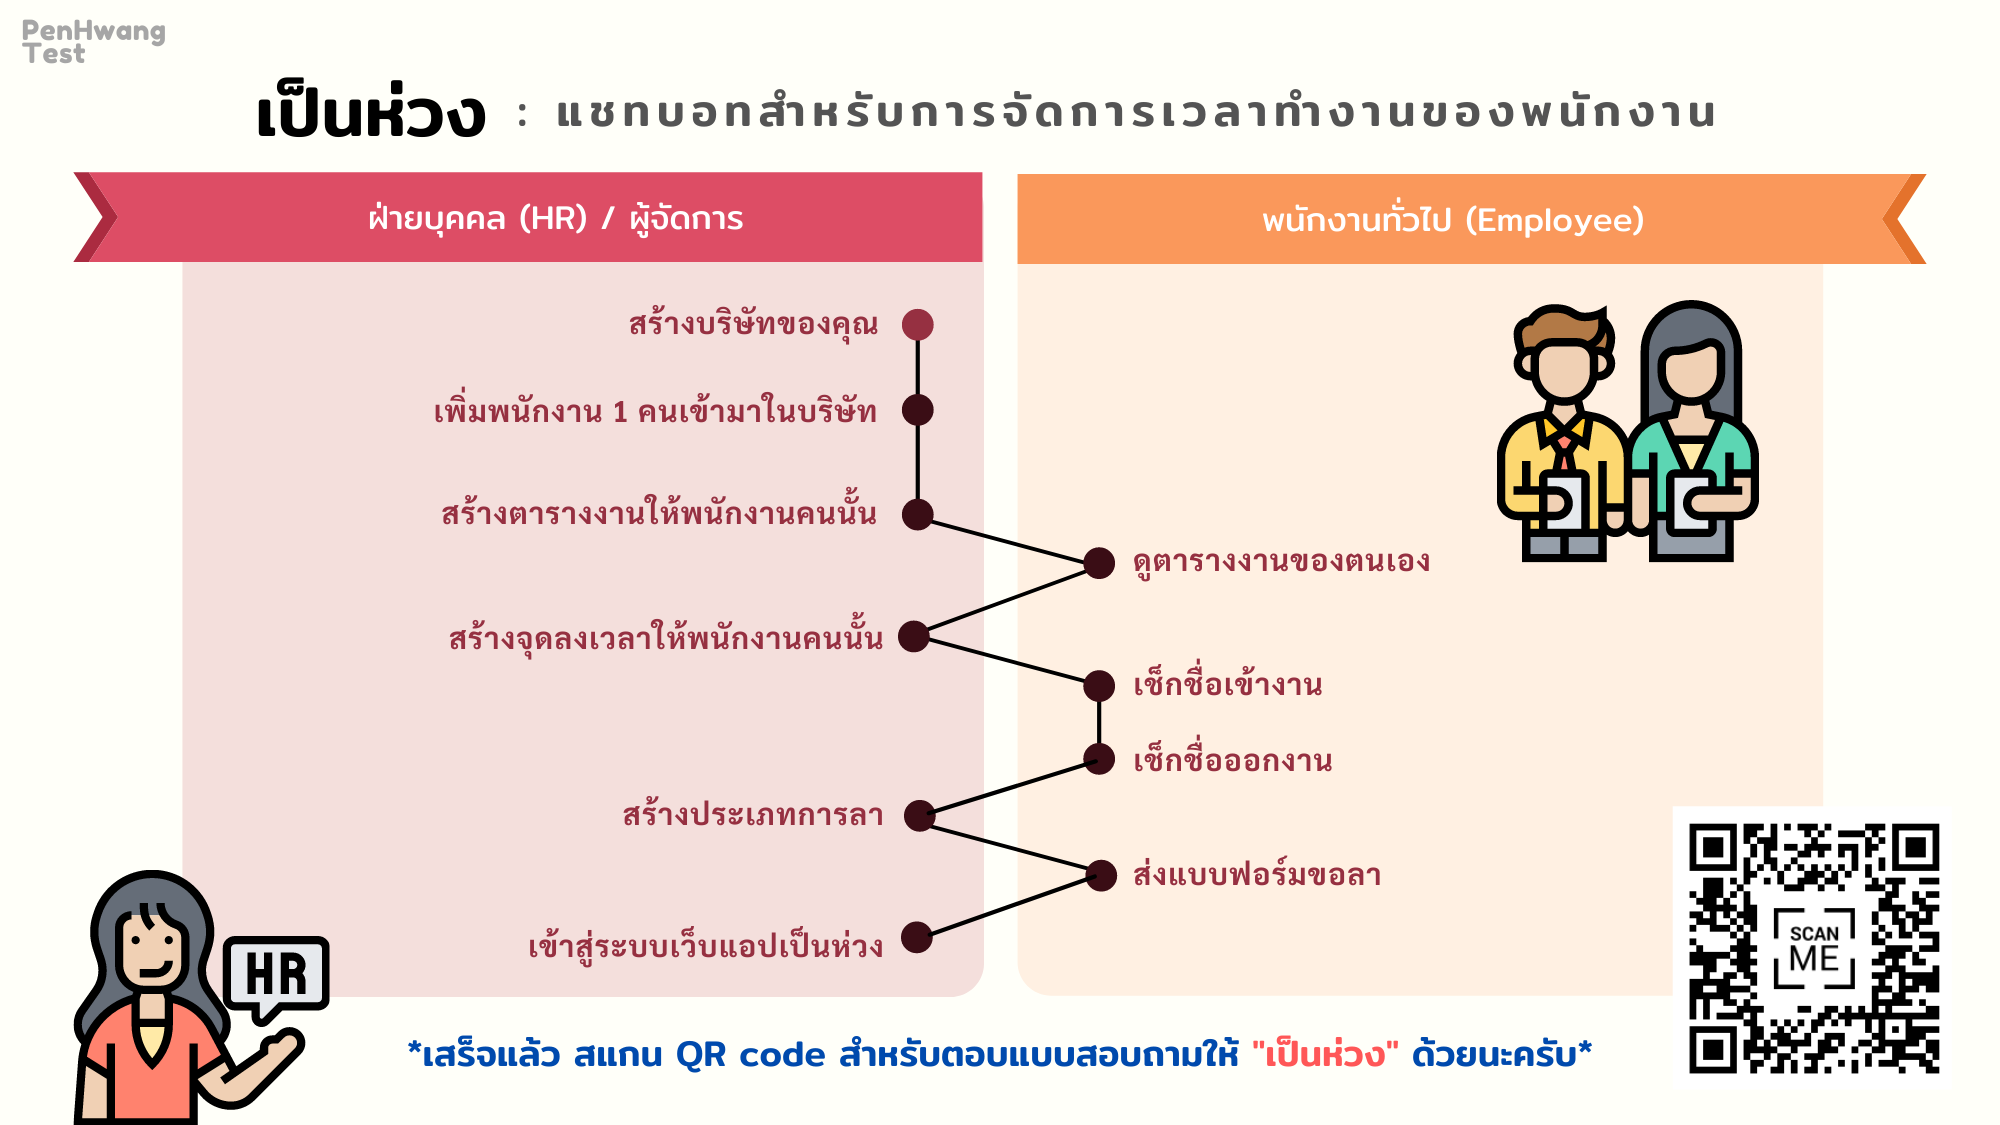
\includegraphics[width=14cm,keepaspectratio]{./images/test_flow.png}
  \end{center}
  \caption[รูปแสดงโจทย์ที่ส่งให้ผู้ทดสอบลองทำตาม]{รูปแสดงโจทย์ที่ส่งให้ผู้ทดสอบลองทำตาม} 
  \label{fig:eval_test}
\end{figure}

\begin{figure}
  \begin{center}
    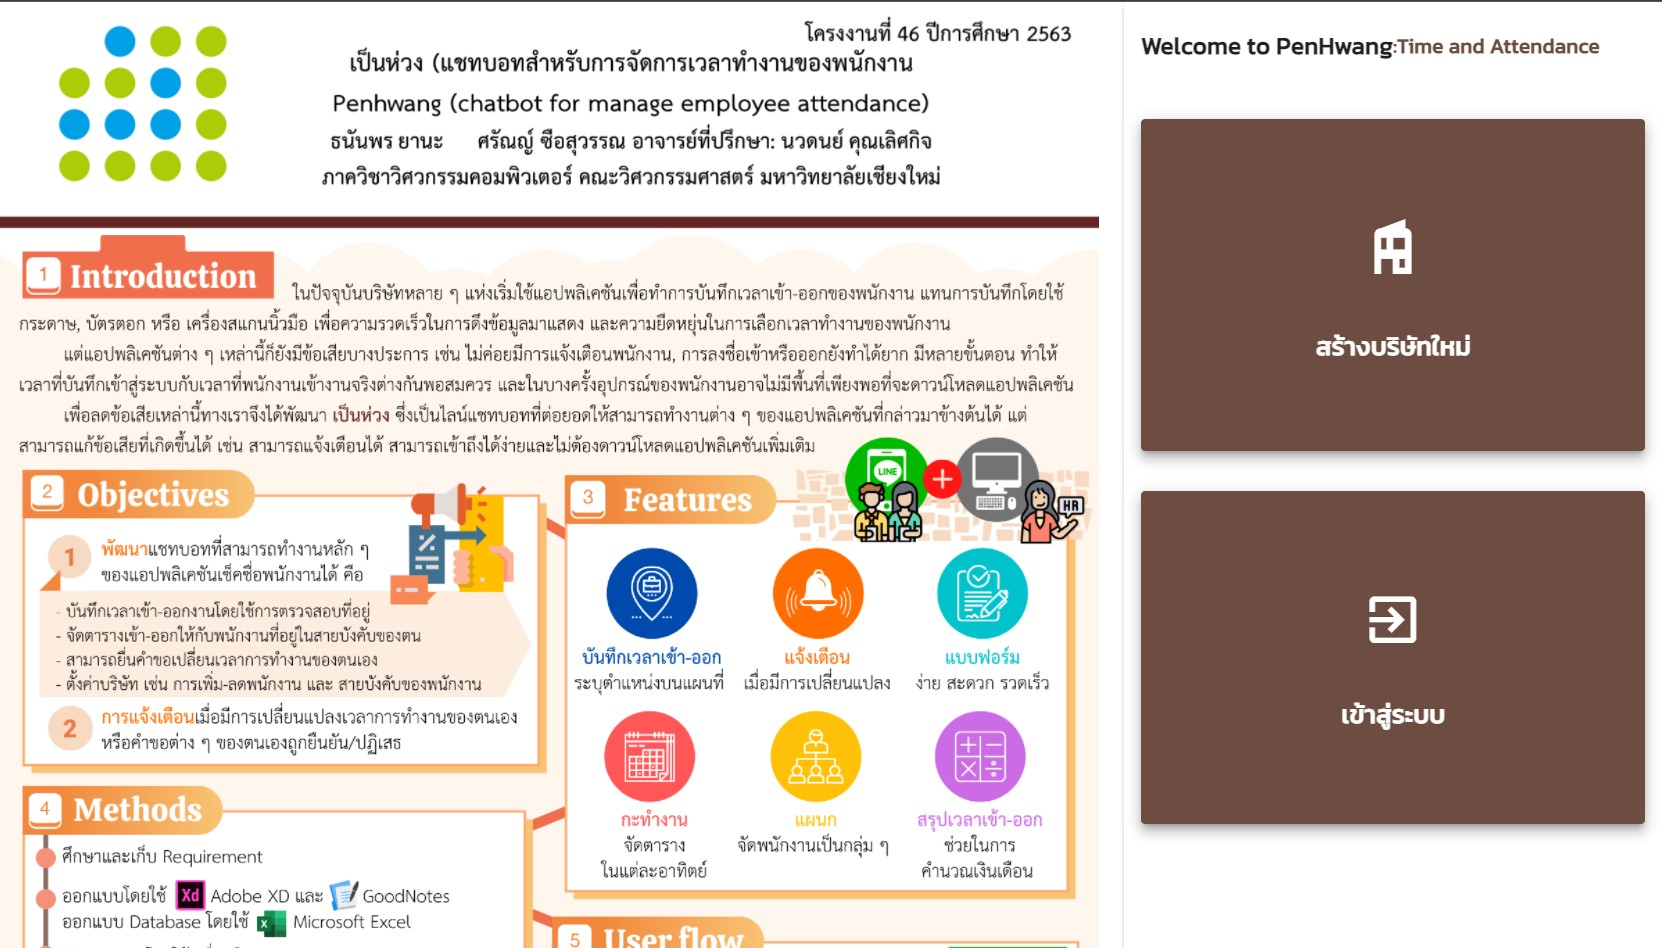
\includegraphics[width=14cm,keepaspectratio]{./images/index.jpg}
  \end{center}
  \caption[รูปแสดงหน้าแรกของเว็บแอปพลิเคชันเป็นห่วง]{รูปแสดงหน้าแรกของเว็บแอปพลิเคชันเป็นห่วง} 
  \label{fig:index}
\end{figure}

\begin{figure}
  \begin{center}
    
\includegraphics[width=7cm,keepaspectratio]{./images/rich_menu.jpg}
  \end{center}
  \caption[รูปแสดง rich menu ใน LINE]{รูปแสดง rich menu ใน LINE} 
  \label{fig:rich_menu}
\end{figure} 

\begin{figure}
  \begin{center}
    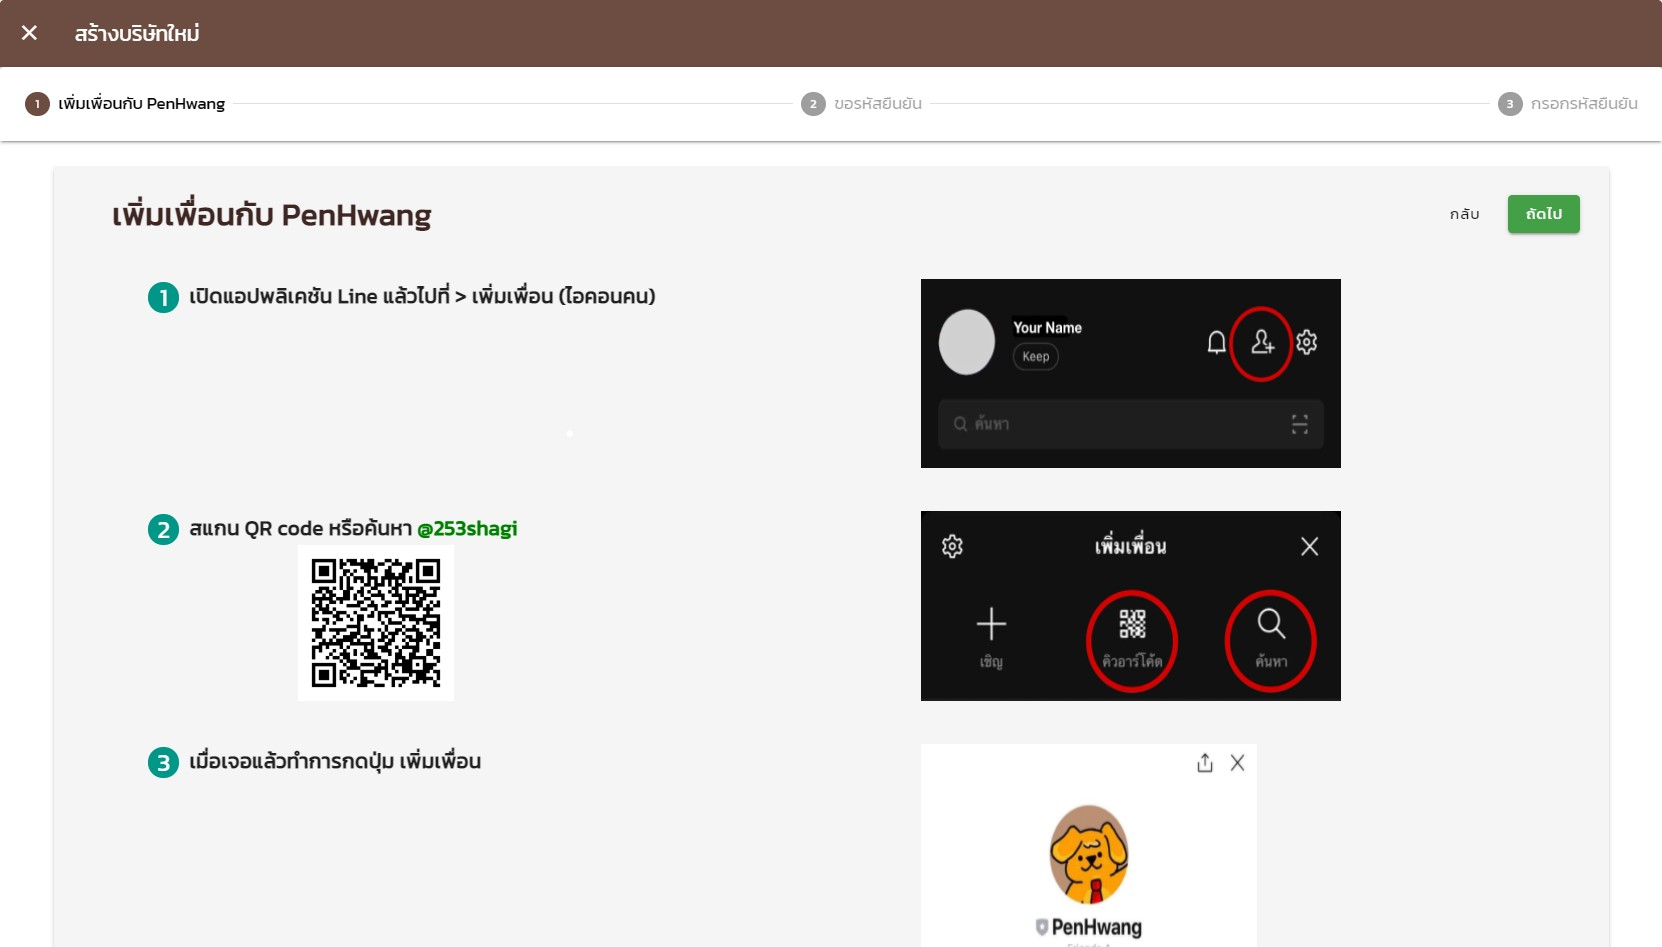
\includegraphics[width=14cm,keepaspectratio]{./images/create_company.jpg}
  \end{center}
  \caption[รูปแสดงวิธีการสร้างบริษัทใหม่]{รูปแสดงวิธีการสร้างบริษัทใหม่} 
  \label{fig:create_company}
\end{figure}

\begin{figure}
  \begin{center}
    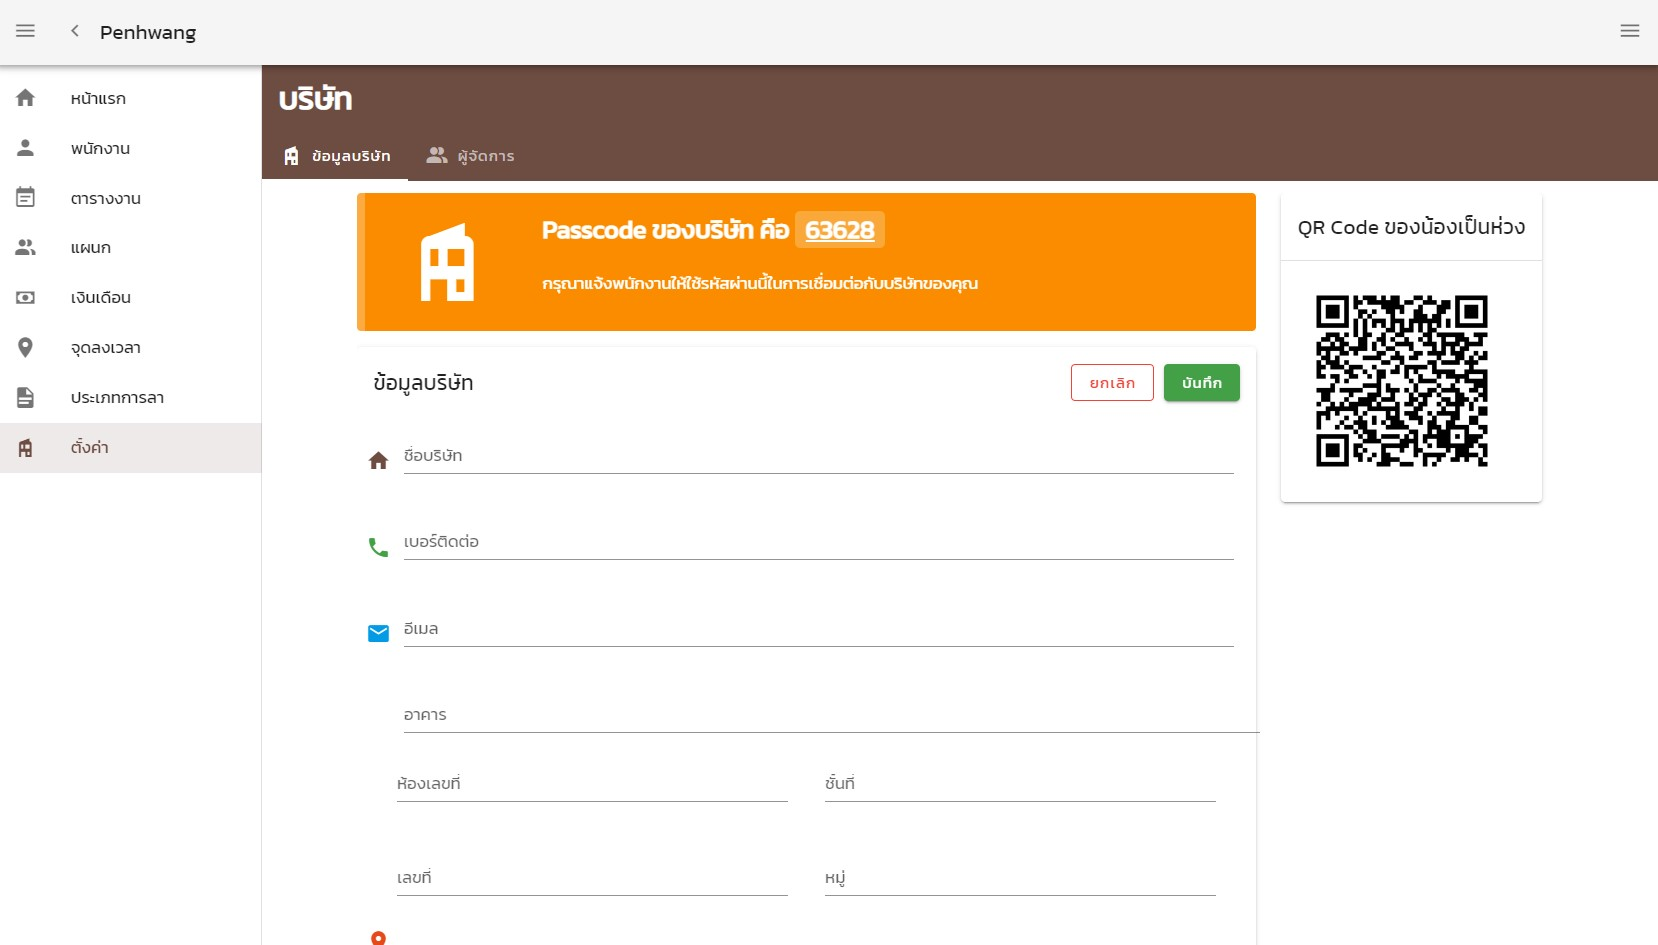
\includegraphics[width=14cm,keepaspectratio]{./images/setting.jpg}
  \end{center}
  \caption[รูปแสดงหน้าตั้งค่าบริษัท]{รูปแสดงหน้าตั้งค่าบริษัท} 
  \label{fig:setting}
\end{figure}

\begin{figure}
  \begin{center}
    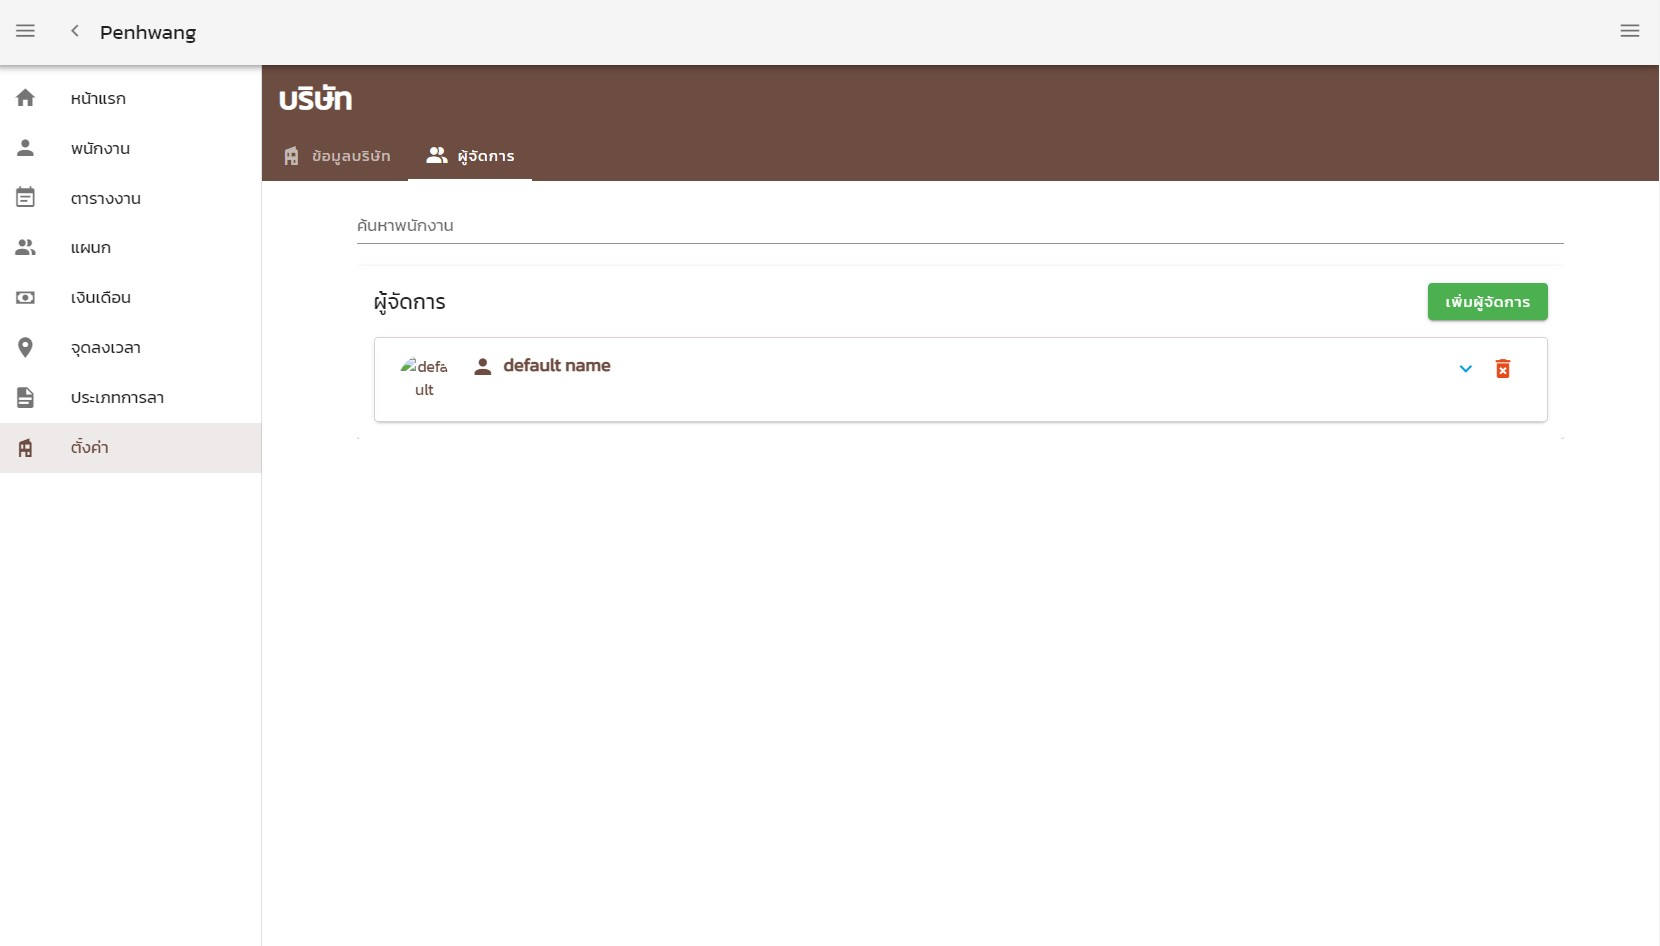
\includegraphics[width=14cm,keepaspectratio]{./images/manager.jpg}
  \end{center}
  \caption[รูปแสดงหน้าจัดการผู้จัดการ/พนักงานฝ่ายบุคคลของบริษัท]{รูปแสดงหน้าจัดการผู้จัดการ/พนักงานฝ่ายบุคคลของบริษัท} 
  \label{fig:manager}
\end{figure}

\begin{figure}
  \begin{center}
    
\includegraphics[width=4cm,keepaspectratio]{./images/message_start_form.jpg}
  \end{center}
  \caption[รูปแสดงข้อความตอบกลับเมื่อขอเป็นพนักงานใหม่]{รูปแสดงข้อความตอบกลับเมื่อขอเป็นพนักงานใหม่} 
  \label{fig:message_start_form}
\end{figure}

\begin{figure}
  \begin{center}
    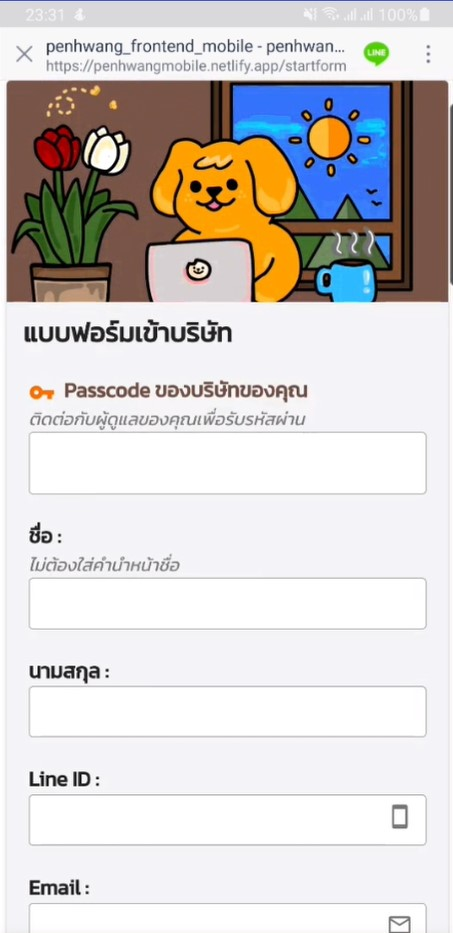
\includegraphics[width=4cm,keepaspectratio]{./images/line_start_form.jpg}
  \end{center}
  \caption[รูปแสดงแบบฟอร์มเข้าร่วมบริษัท]{รูปแสดงแบบฟอร์มเข้าร่วมบริษัท} 
  \label{fig:line_start_form}
\end{figure}

\begin{figure}
  \begin{center}
    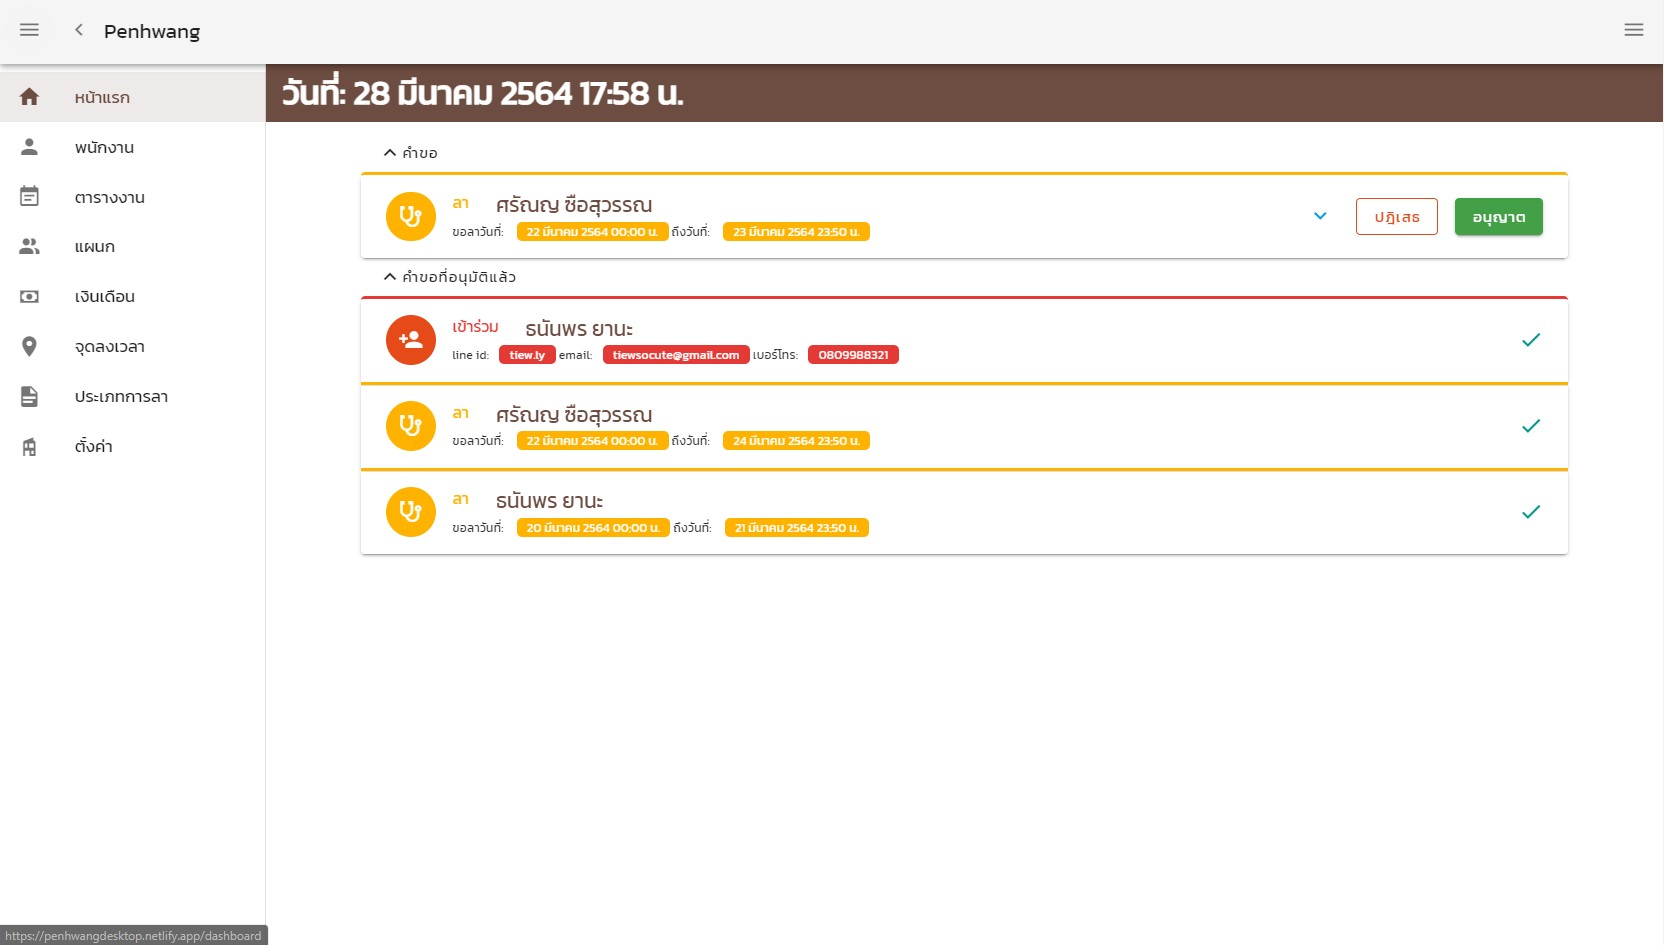
\includegraphics[width=14cm,keepaspectratio]{./images/dashboard.jpg}
  \end{center}
  \caption[รูปแสดงหน้าสรุปคำขอจากพนักงาน]{รูปแสดงหน้าสรุปคำขอจากพนักงาน} 
  \label{fig:dashboard}
\end{figure}

\begin{figure}
  \begin{center}
    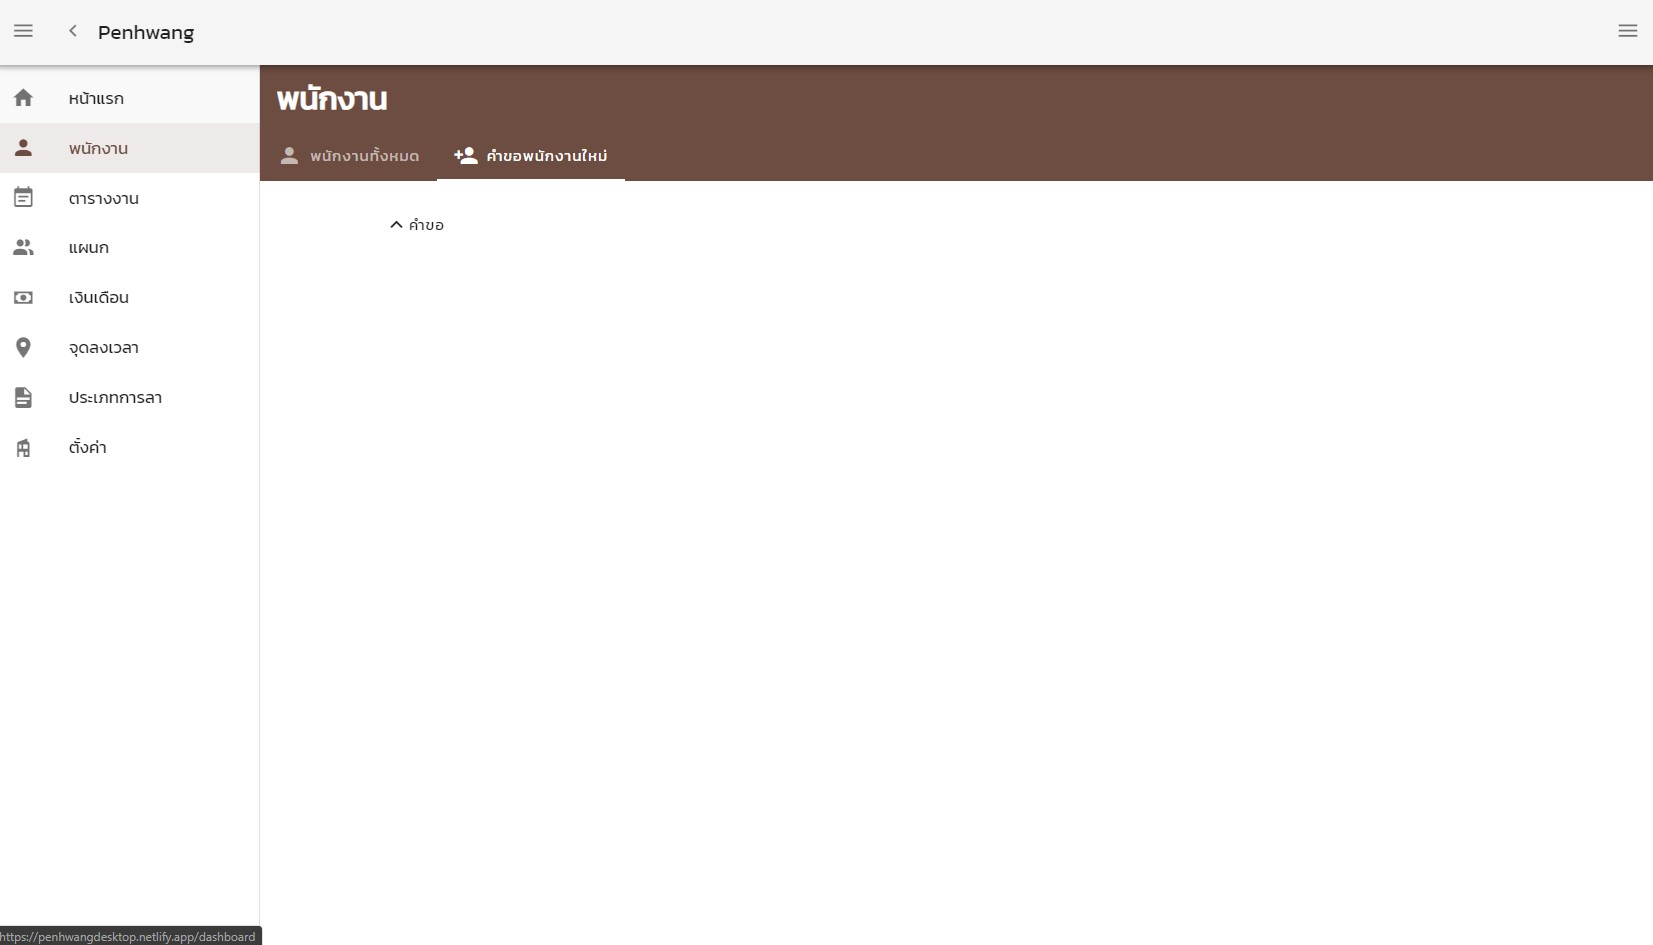
\includegraphics[width=14cm,keepaspectratio]{./images/new_employee.jpg}
  \end{center}
  \caption[รูปแสดงหน้าพนักงานใหม่]{รูปแสดงหน้าพนักงานใหม่} 
  \label{fig:new_employee}
\end{figure}

\begin{figure}
  \begin{center}
    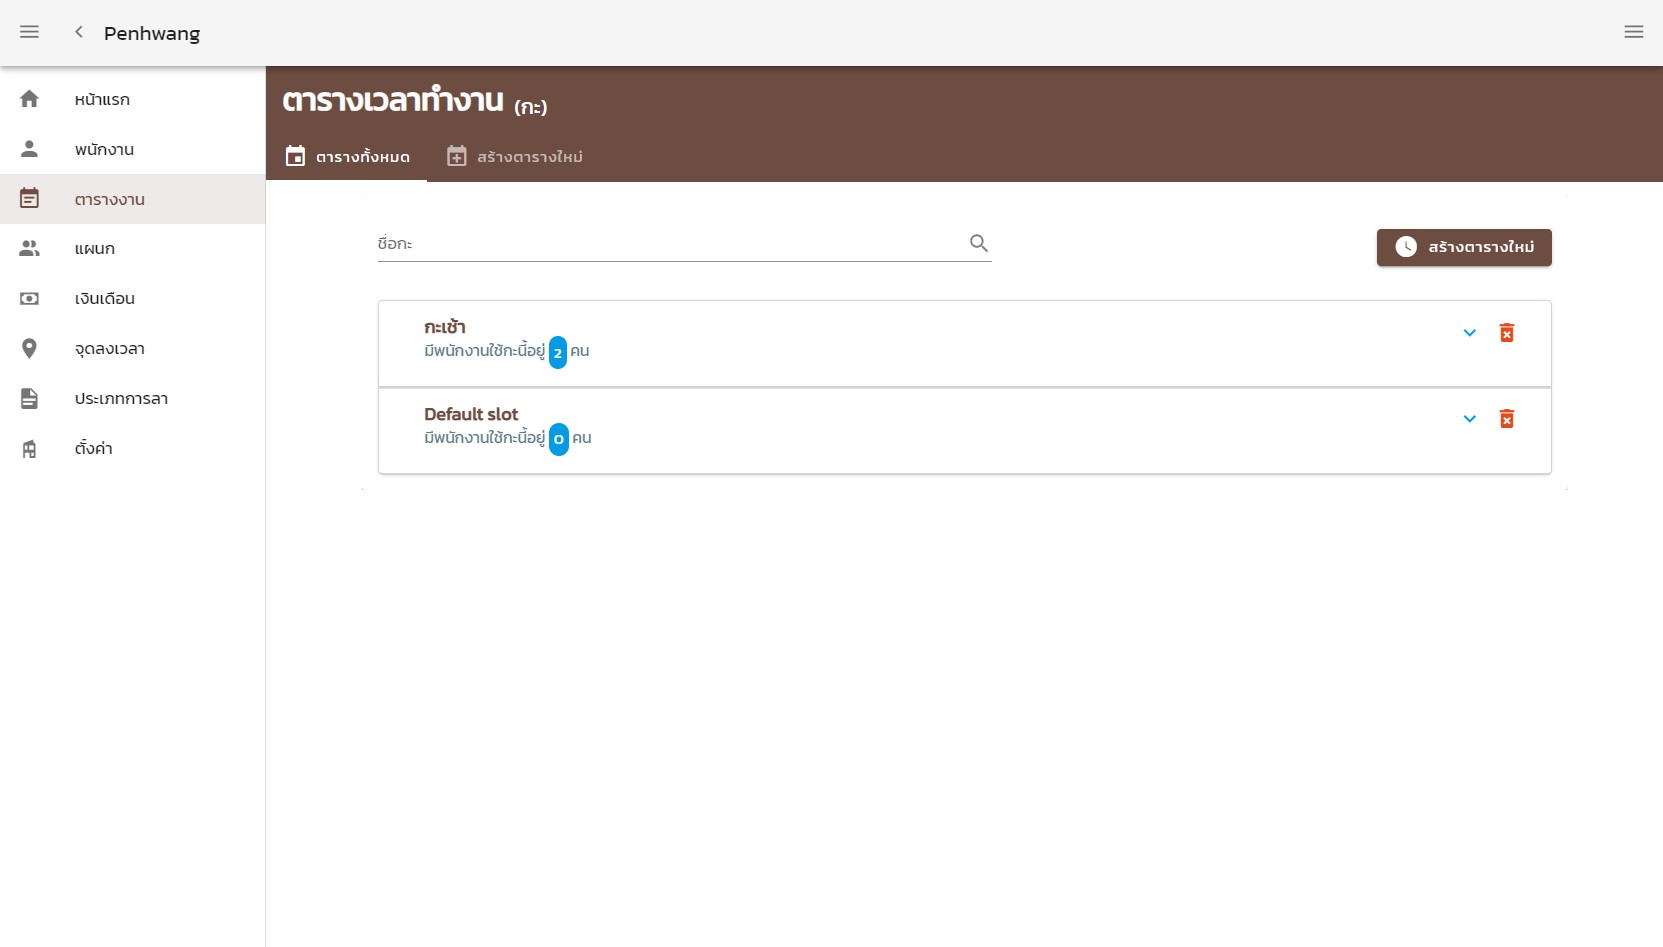
\includegraphics[width=14cm,keepaspectratio]{./images/slot.jpg}
  \end{center}
  \caption[รูปแสดงหน้ารวมของตารางเวลาทำงาน/กะ]{รูปแสดงหน้ารวมของตารางเวลาทำงาน/กะ} 
  \label{fig:slot}
\end{figure}
 
\begin{figure}
  \begin{center}
    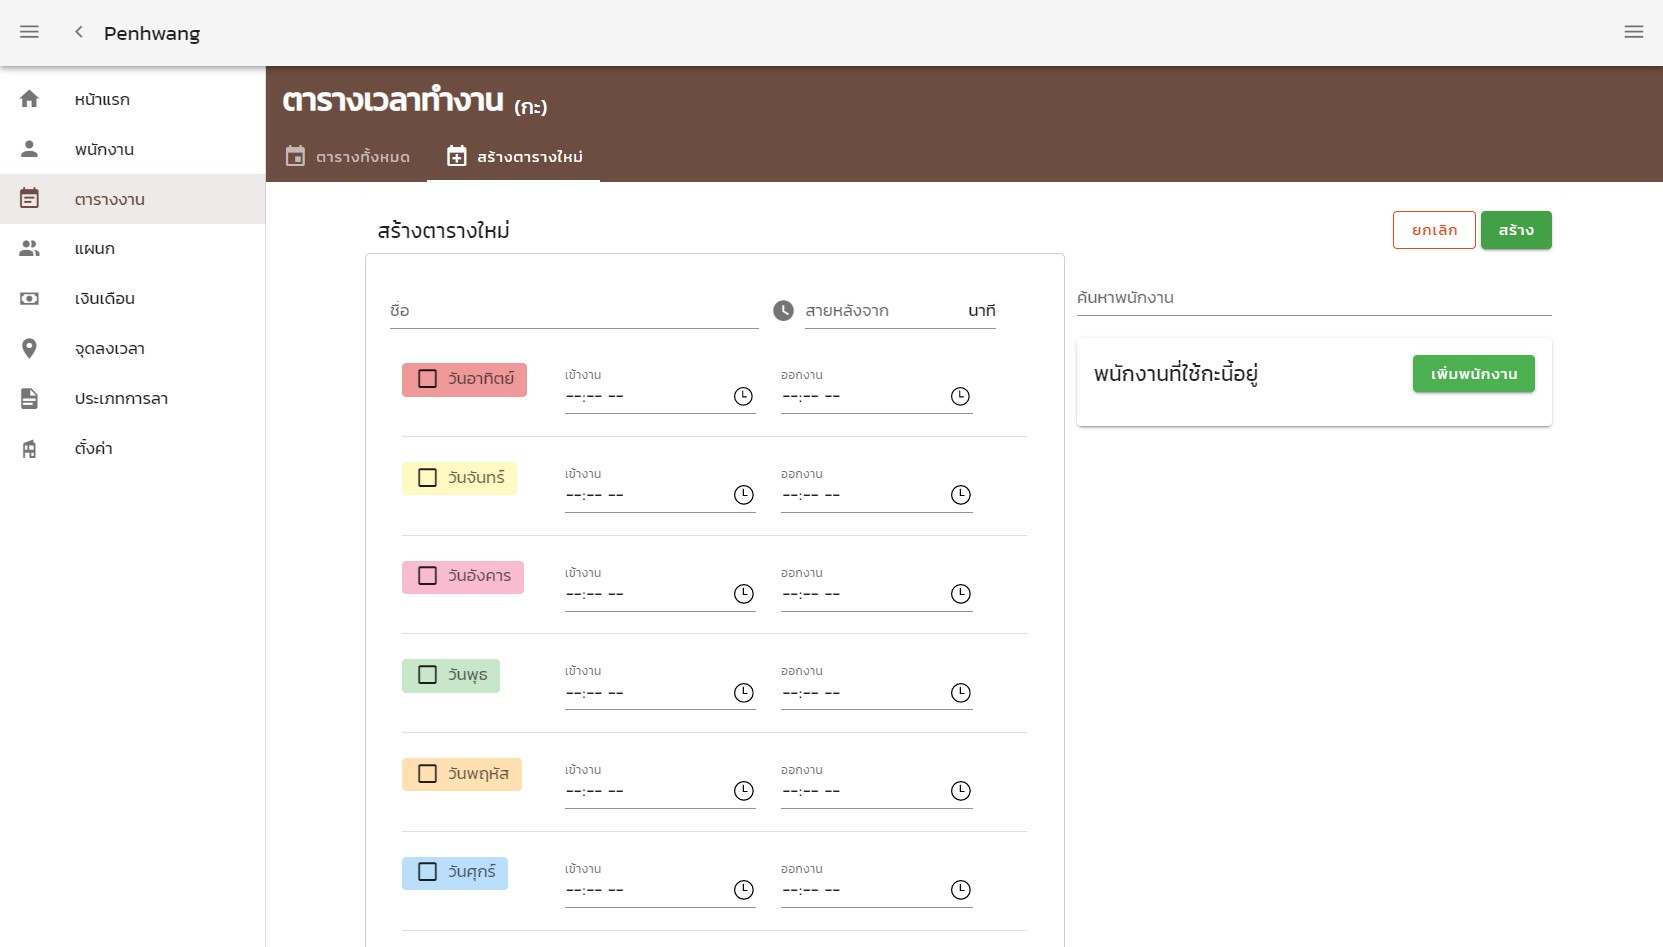
\includegraphics[width=14cm,keepaspectratio]{./images/new_slot.jpg}
  \end{center}
  \caption[รูปแสดงหน้าสร้างกะใหม่]{รูปแสดงหน้าสร้างกะใหม่} 
  \label{fig:new_slot}
\end{figure}
 
\begin{figure}
  \begin{center}
    
\includegraphics[width=4cm,keepaspectratio]{./images/added_slot.jpg}
  \end{center}
  \caption[รูปแสดงข้อความเมื่อกะมีการเปลี่ยนแปลง]{รูปแสดงข้อความเมื่อกะมีการเปลี่ยนแปลง} 
  \label{fig:added_slot}
\end{figure}

\begin{figure}
  \begin{center}
    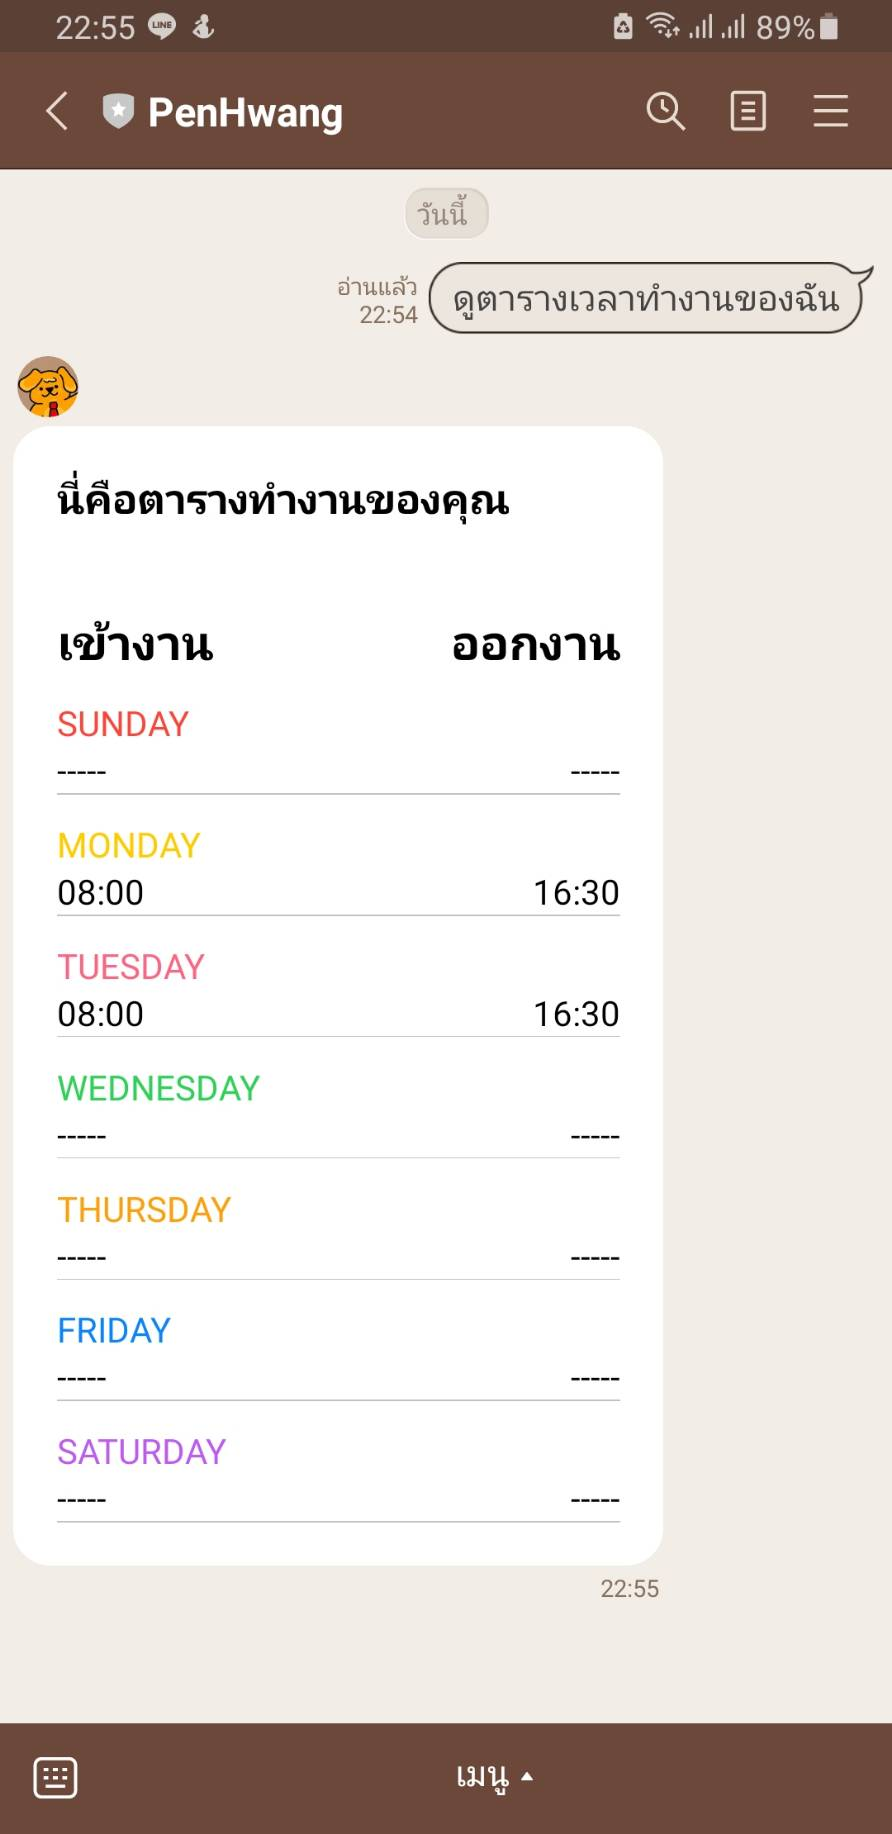
\includegraphics[width=4cm,keepaspectratio]{./images/message_slot.jpg}
  \end{center}
  \caption[รูปแสดงข้อความบอกตารางเวลาทำงานของพนักงาน]{รูปแสดงข้อความบอกตารางเวลาทำงานของพนักงาน} 
  \label{fig:message_slot}
\end{figure}

\begin{figure}
  \begin{center}
    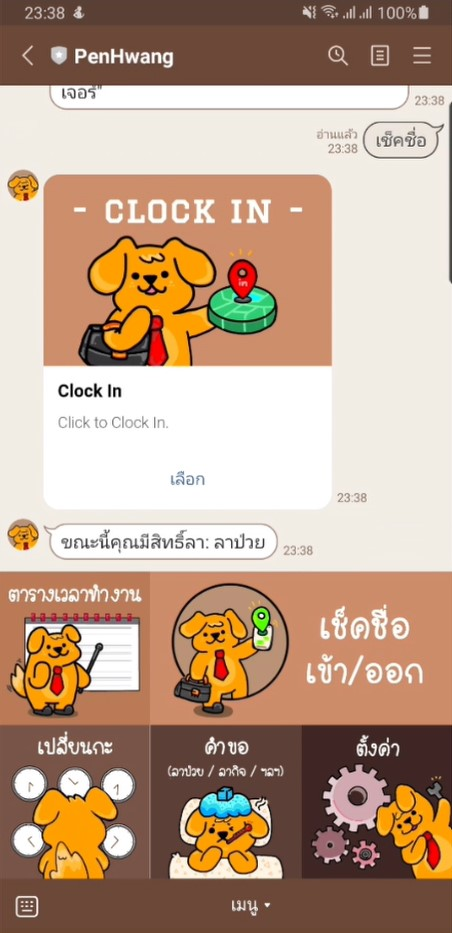
\includegraphics[width=4cm,keepaspectratio]{./images/added_leave.jpg}
  \end{center}
  \caption[รูปแสดงข้อความเมื่อมีการเพิ่ม/ยกเลิกประเภทการลาของพนักงาน]{รูปแสดงข้อความเมื่อมีการเพิ่ม/ยกเลิกประเภทการลาของพนักงาน} 
  \label{fig:added_leave}
\end{figure}

\begin{figure}
  \begin{center}
    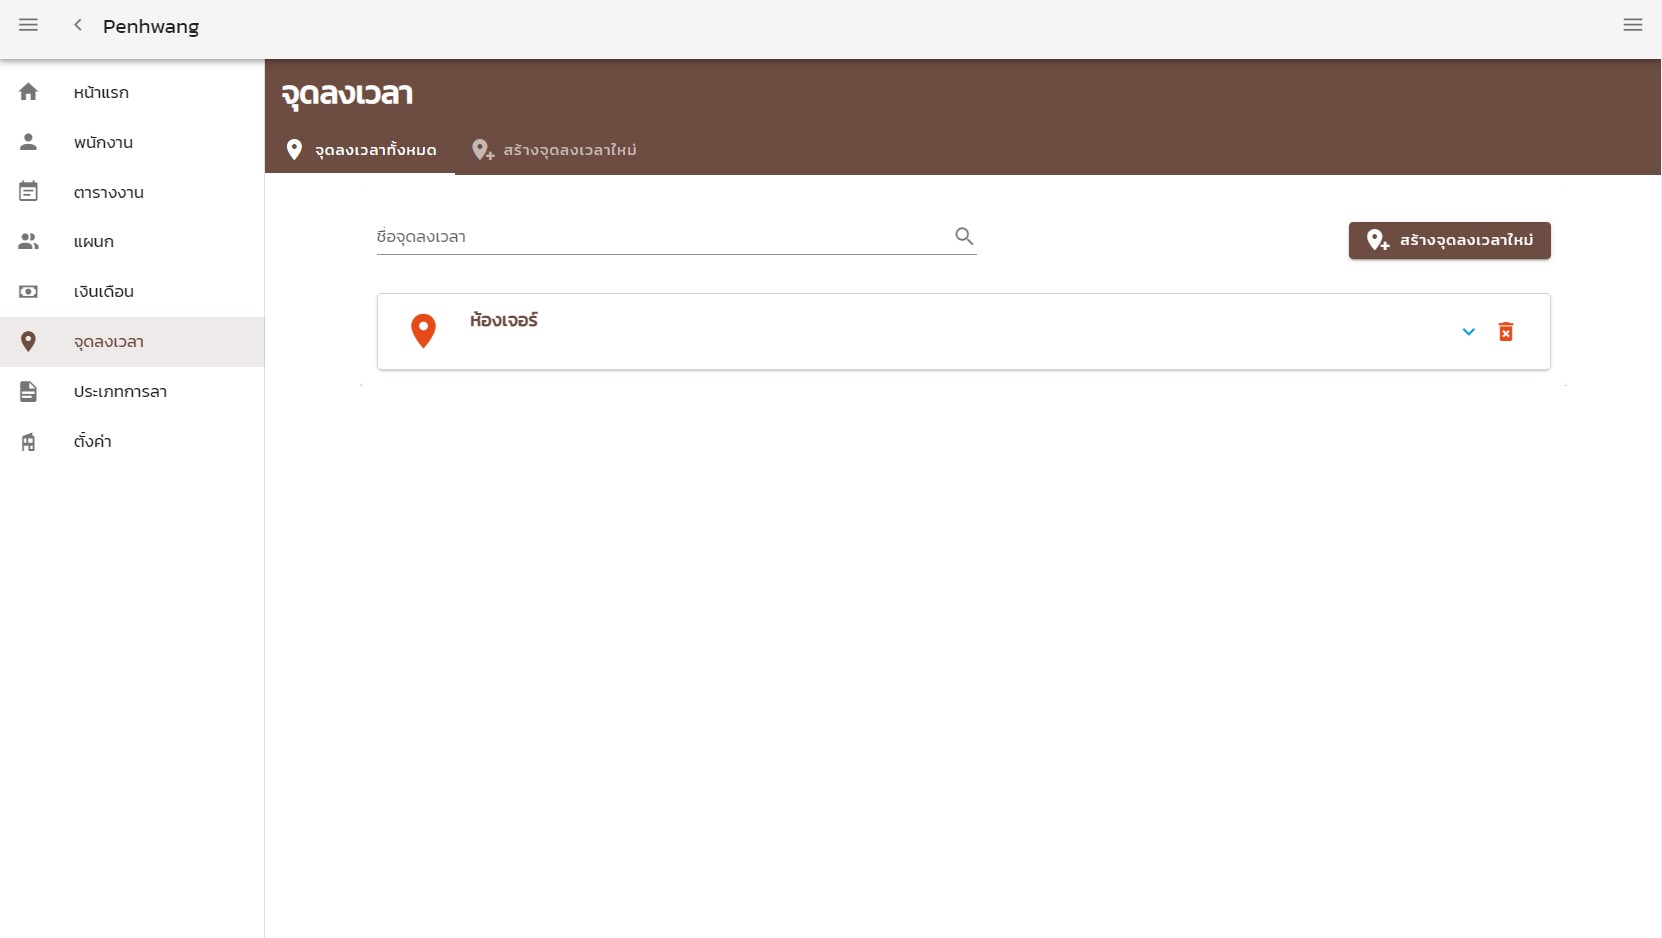
\includegraphics[width=14cm,keepaspectratio]{./images/location.jpg}
  \end{center}
  \caption[รูปแสดงหน้ารวมของจุดลงเวลา]{รูปแสดงหน้ารวมของจุดลงเวลา} 
  \label{fig:location}
\end{figure}
 
\begin{figure}
  \begin{center}
    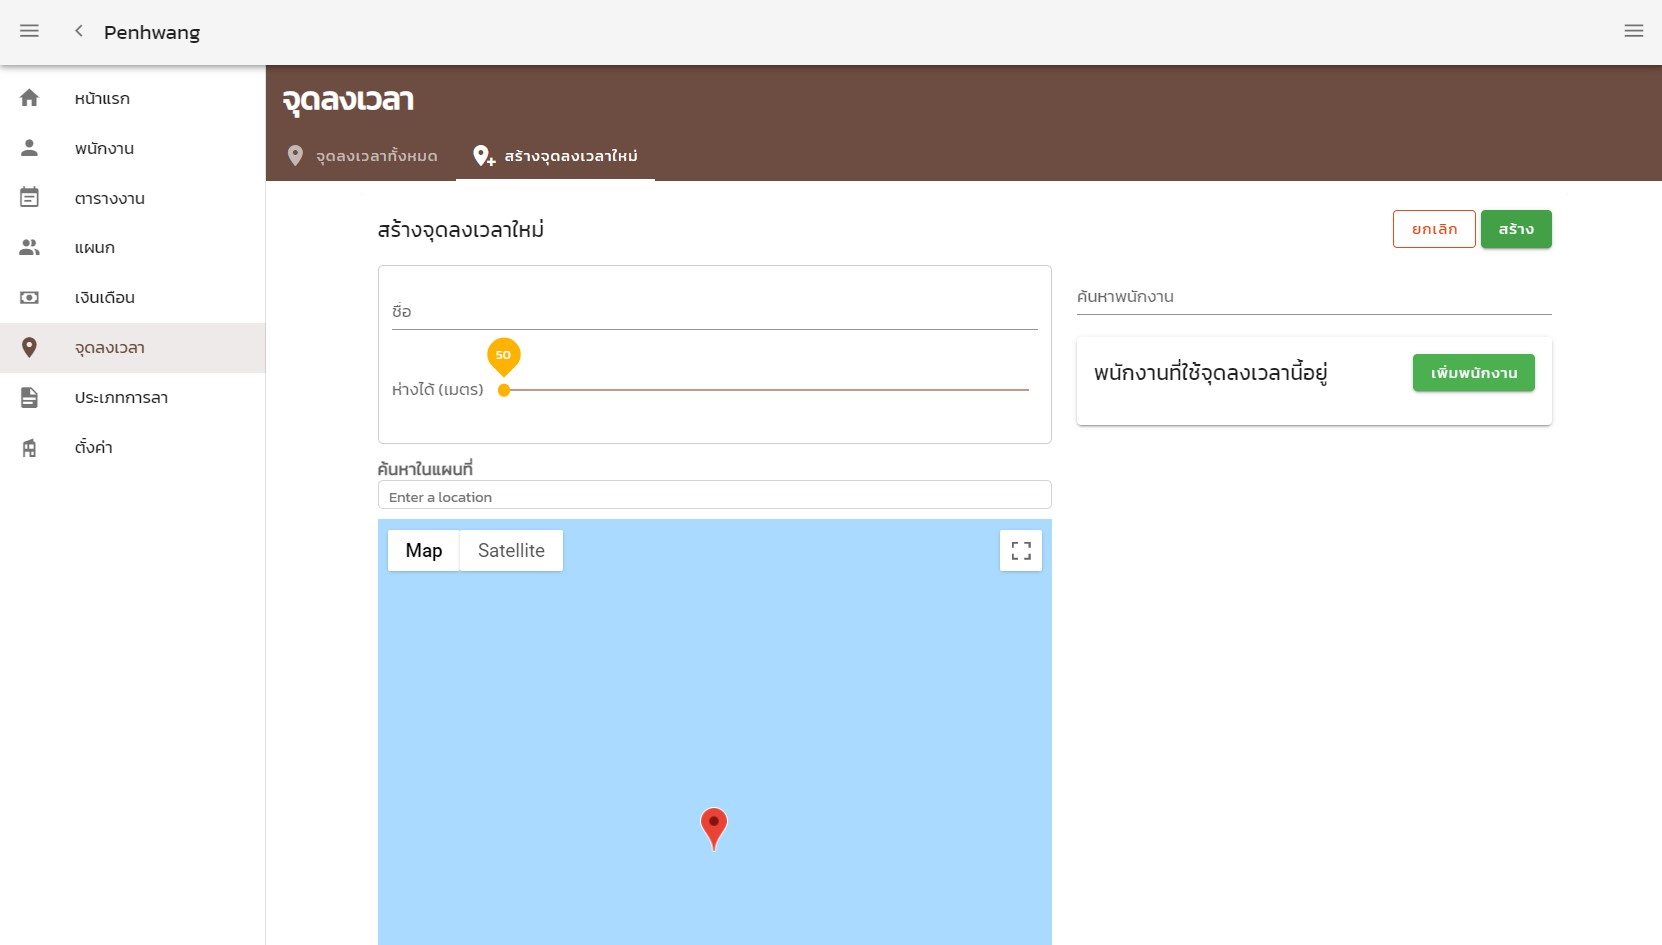
\includegraphics[width=14cm,keepaspectratio]{./images/new_location.jpg}
  \end{center}
  \caption[รูปแสดงหน้าสร้างจุดลงเวลาใหม่]{รูปแสดงหน้าสร้างจุดลงเวลาใหม่} 
  \label{fig:new_location}
\end{figure}
 
\begin{figure}
  \begin{center}
    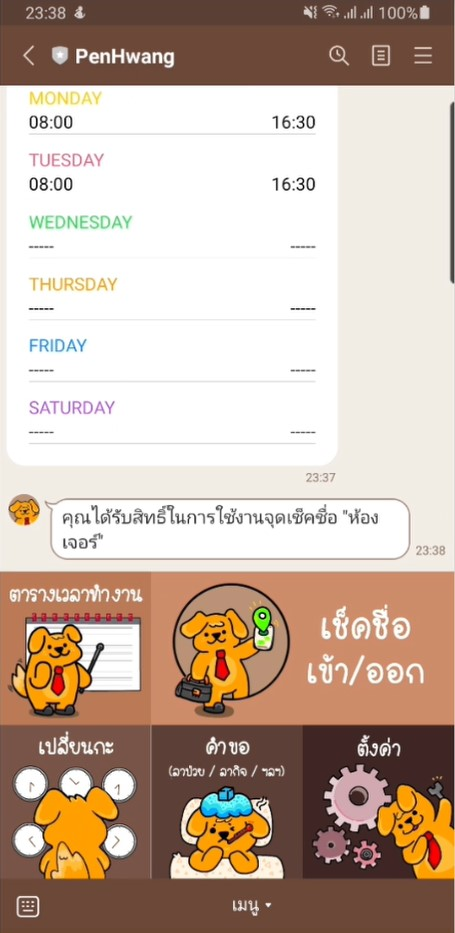
\includegraphics[width=4cm,keepaspectratio]{./images/added_location.jpg}
  \end{center}
  \caption[รูปแสดงข้อความเมื่อได้รับสิทธิ์ในการลงเวลาที่จุดลงเวลาใหม่]{รูปแสดงข้อความเมื่อได้รับสิทธิ์ในการลงเวลาที่จุดลงเวลาใหม่} 
  \label{fig:added_location}
\end{figure}

\begin{figure}
  \begin{center}
    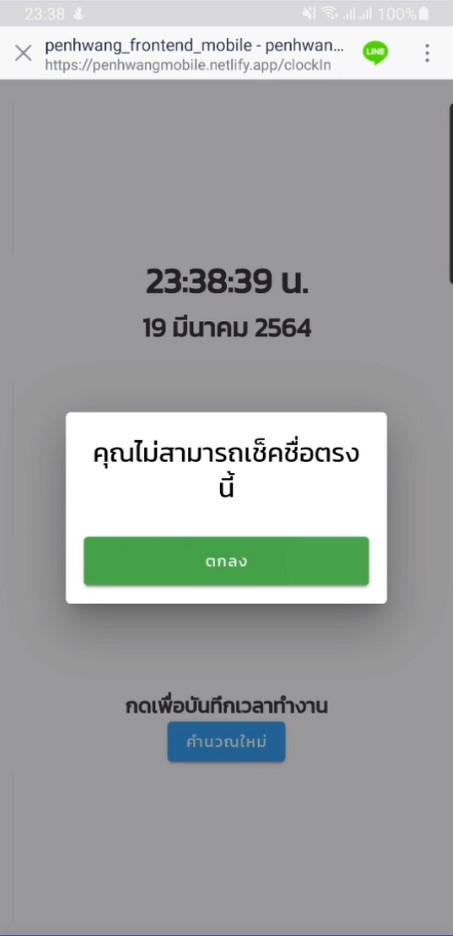
\includegraphics[width=4cm,keepaspectratio]{./images/cant_clock.jpg}
  \end{center}
  \caption[รูปแสดงข้อความเมื่อไม่สามารถลงเวลา ณ จุดนี้ได้]{รูปแสดงข้อความเมื่อไม่สามารถลงเวลา ณ จุดนี้ได้} 
  \label{fig:cant_clock}
\end{figure}
 
\begin{figure}
  \begin{center}
    
\includegraphics[width=4cm,keepaspectratio]{./images/clock.jpg}
  \end{center}
  \caption[รูปแสดงหน้าจอ เมื่อสามารถลงเวลา ณ จุดนี้ได้]{รูปแสดงหน้าจอ เมื่อสามารถลงเวลา ณ จุดนี้ได้} 
  \label{fig:clock}
\end{figure}

\begin{figure}
  \begin{center}
    
\includegraphics[width=4cm,keepaspectratio]{./images/clock_in.jpg}
  \end{center}
  \caption[รูปแสดงข้อความตอบกลับเมื่อขอเข้างาน]{รูปแสดงข้อความตอบกลับเมื่อขอเข้างาน} 
  \label{fig:clock_in}
\end{figure}
 
\begin{figure}
  \begin{center}
    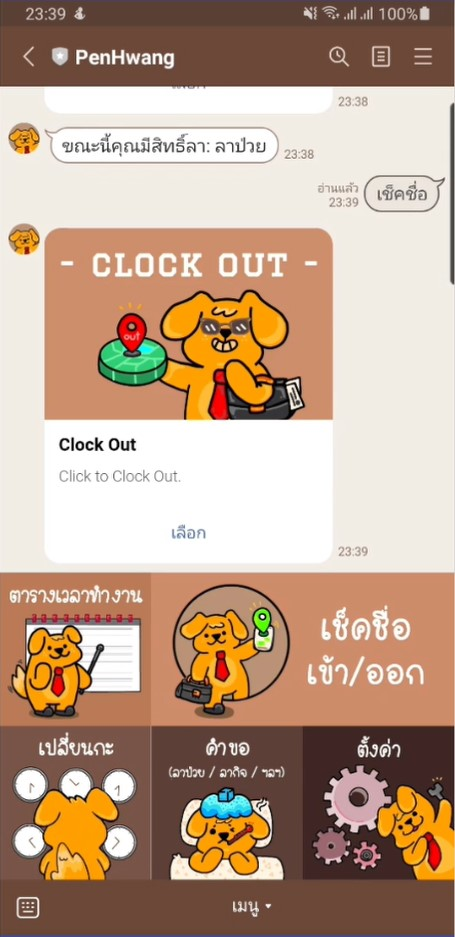
\includegraphics[width=4cm,keepaspectratio]{./images/clock_out.jpg}
  \end{center}
  \caption[รูปแสดงข้อความตอบกลับเมื่อขอออกงาน]{รูปแสดงข้อความตอบกลับเมื่อขอออกงาน} 
  \label{fig:clock_out}
\end{figure}
 
\begin{figure}
  \begin{center}
    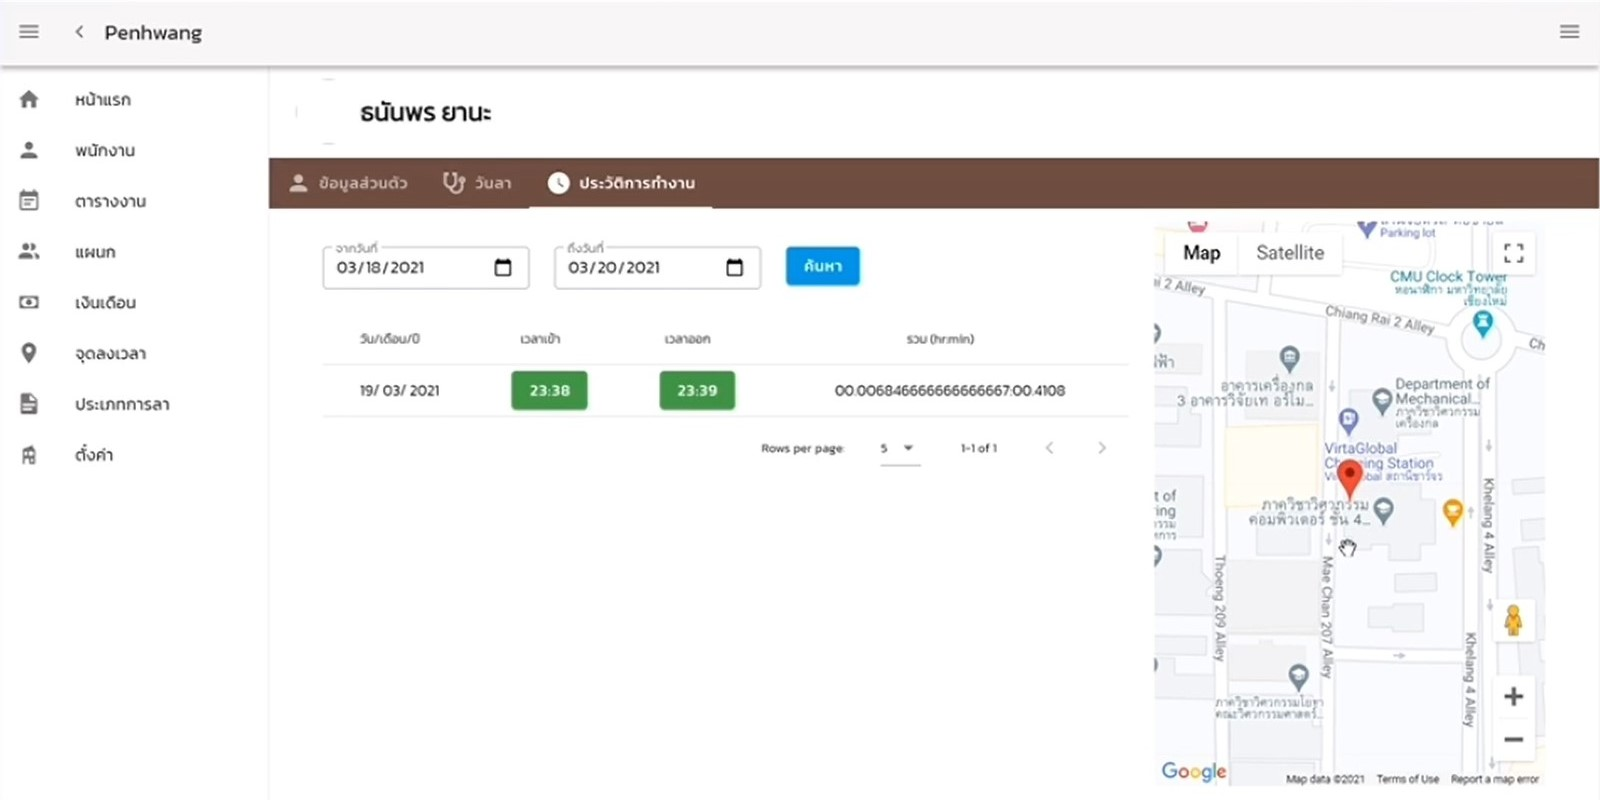
\includegraphics[width=14cm,keepaspectratio]{./images/history.jpg}
  \end{center}
  \caption[รูปแสดงหน้าประวัติการทำงานของพนักงาน]{รูปแสดงหน้าประวัติการทำงานของพนักงาน} 
  \label{fig:history}
\end{figure}

\begin{figure}
  \begin{center}
    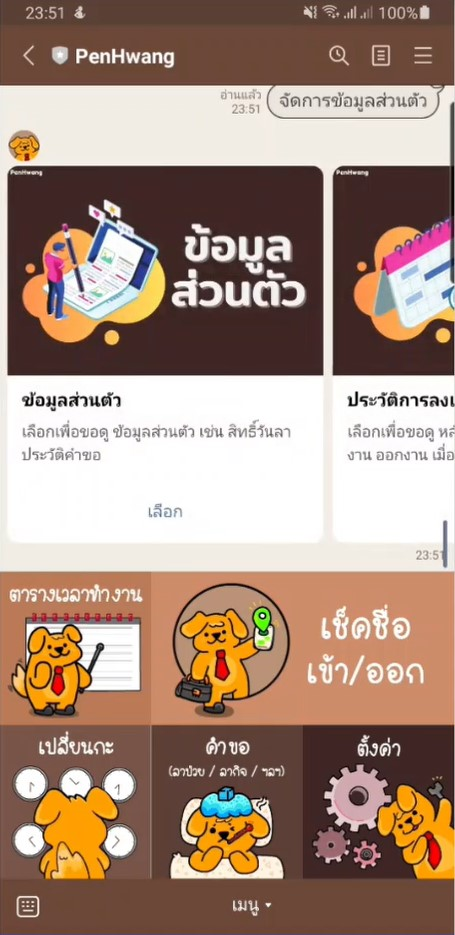
\includegraphics[width=4cm,keepaspectratio]{./images/message_setting.jpg}
  \end{center}
  \caption[รูปแสดงข้อความตอบกลับเมื่อขอตั้งค่า]{รูปแสดงข้อความตอบกลับเมื่อขอตั้งค่า} 
  \label{fig:message_setting}
\end{figure}

\begin{figure}
  \begin{center}
    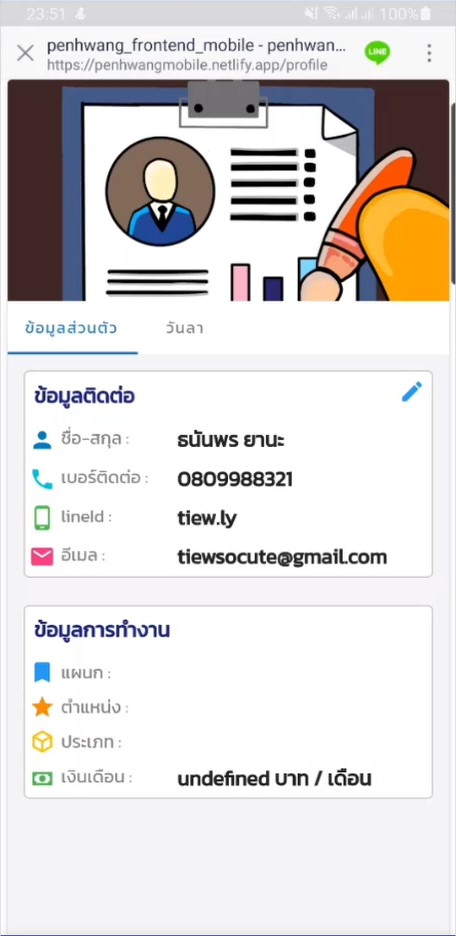
\includegraphics[width=4cm,keepaspectratio]{./images/line_personal_info.jpg}
  \end{center}
  \caption[รูปแสดงหน้าข้อมูลส่วนตัวในโทรศัพท์]{รูปแสดงหน้าข้อมูลส่วนตัวในโทรศัพท์} 
  \label{fig:line_personal_info}
\end{figure} 
 
\begin{figure}
  \begin{center}
    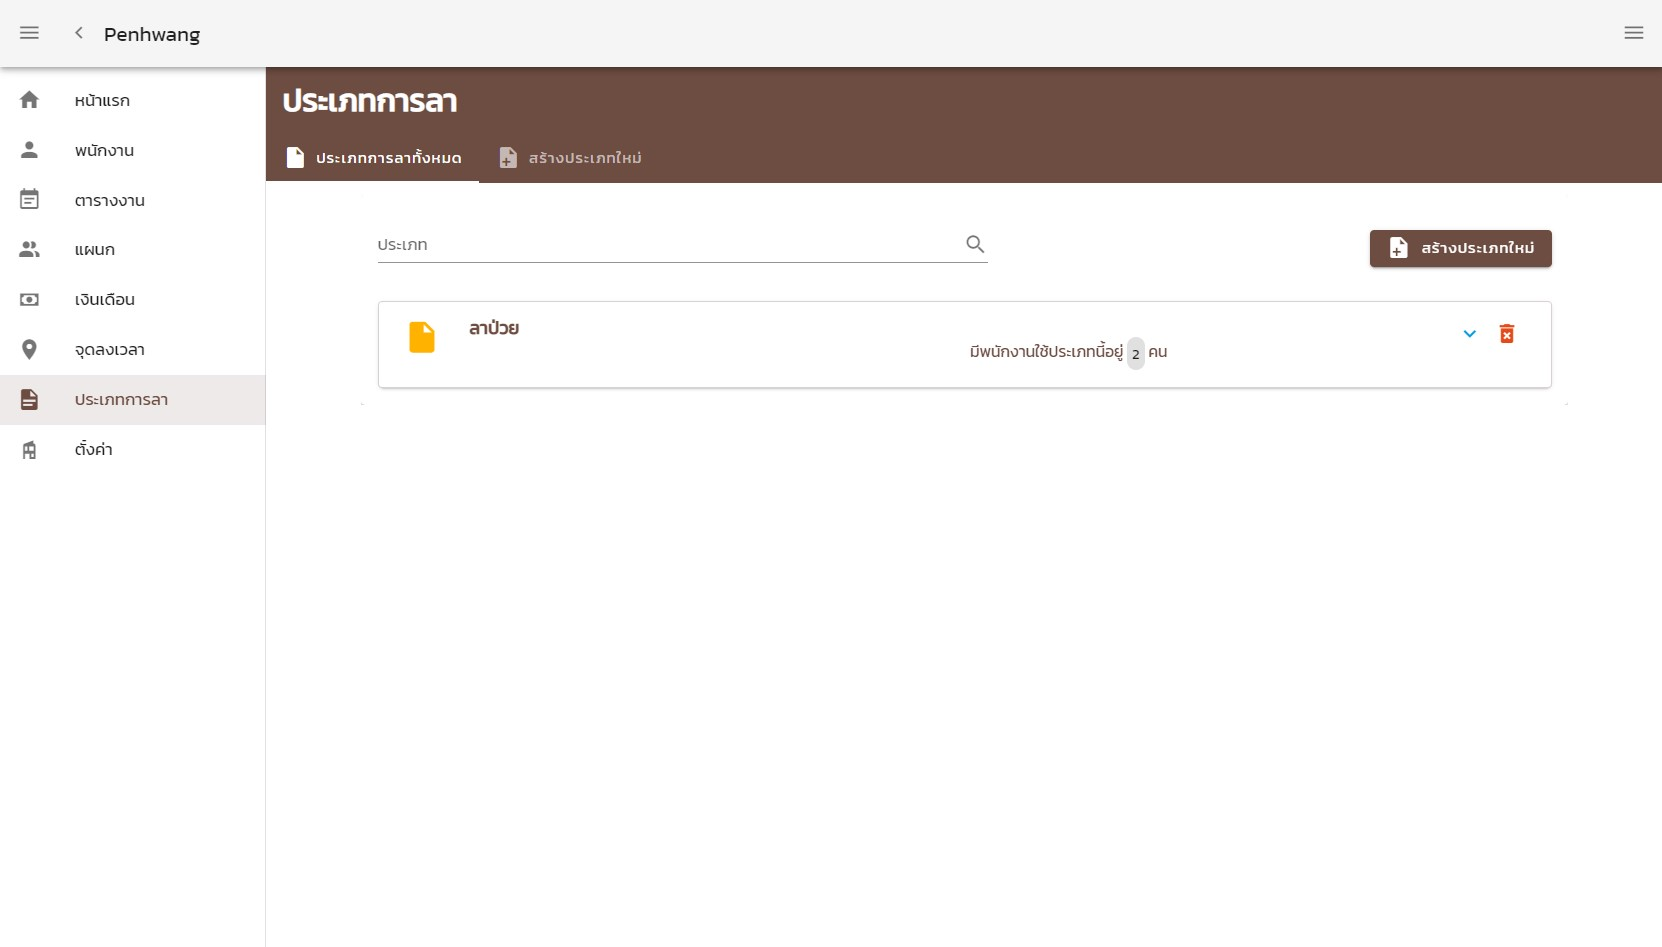
\includegraphics[width=14cm,keepaspectratio]{./images/leave.jpg}
  \end{center}
  \caption[รูปแสดงหน้ารวมของประเภทการลา]{รูปแสดงหน้ารวมของประเภทการลา} 
  \label{fig:leave}
\end{figure}

\begin{figure}
  \begin{center}
    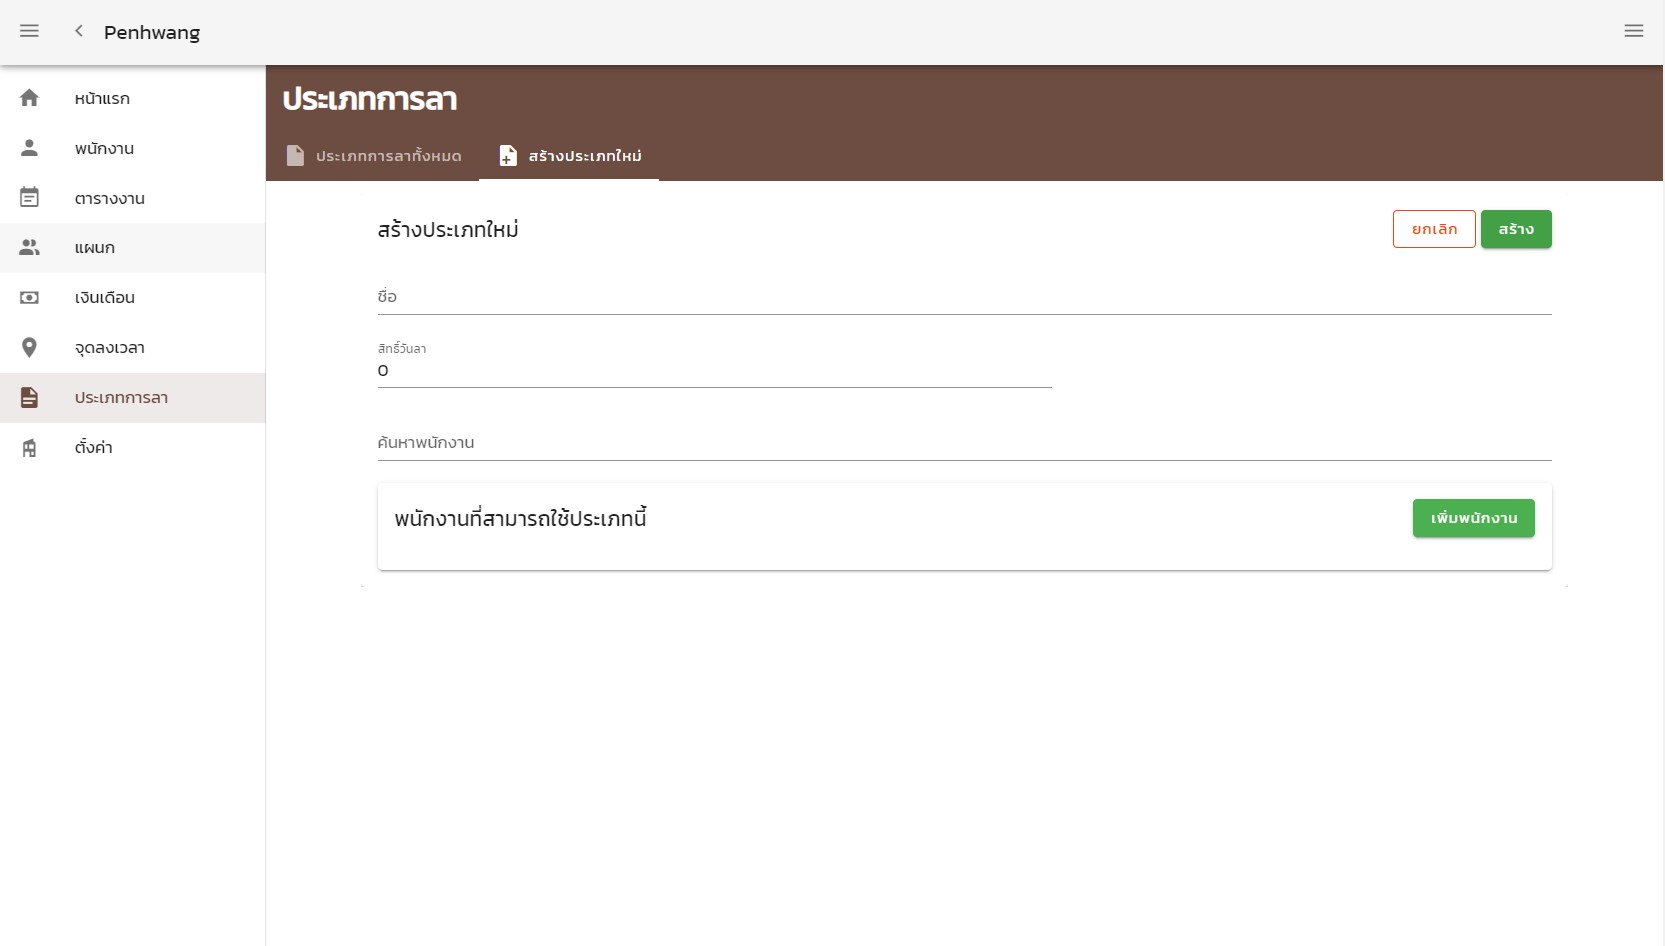
\includegraphics[width=14cm,keepaspectratio]{./images/new_leave.jpg}
  \end{center}
  \caption[รูปแสดงหน้าสร้างประเภทการลาใหม่]{รูปแสดงหน้าสร้างประเภทการลาใหม่} 
  \label{fig:new_leave}
\end{figure} 

\begin{figure}
  \begin{center}
    
\includegraphics[width=4cm,keepaspectratio]{./images/message_leave.jpg}
  \end{center}
  \caption[รูปแสดงข้อความตอบกลับเมื่อขอลา]{รูปแสดงข้อความตอบกลับเมื่อขอลา} 
  \label{fig:message_leave}
\end{figure}
 
\begin{figure}
  \begin{center}
    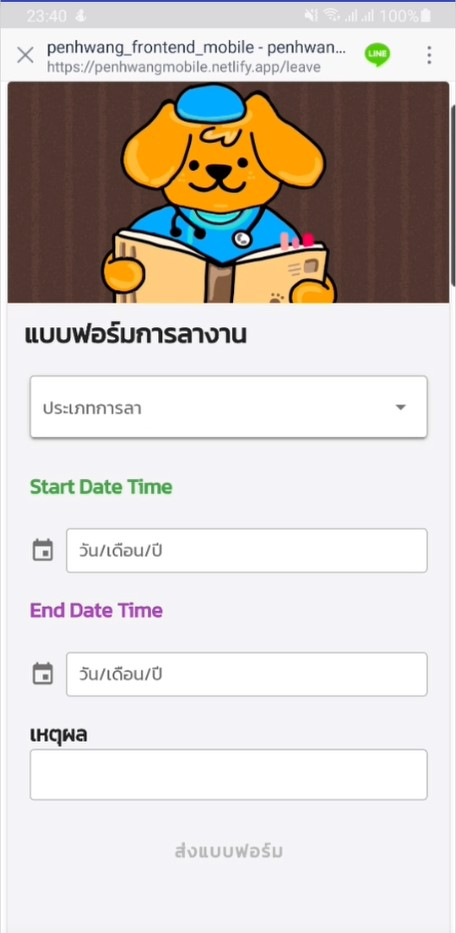
\includegraphics[width=4cm,keepaspectratio]{./images/line_leave.jpg}
  \end{center}
  \caption[รูปแสดงแบบฟอร์มขอลา]{รูปแสดงแบบฟอร์มขอลา} 
  \label{fig:line_leave}
\end{figure}
 
\begin{figure}
  \begin{center}
    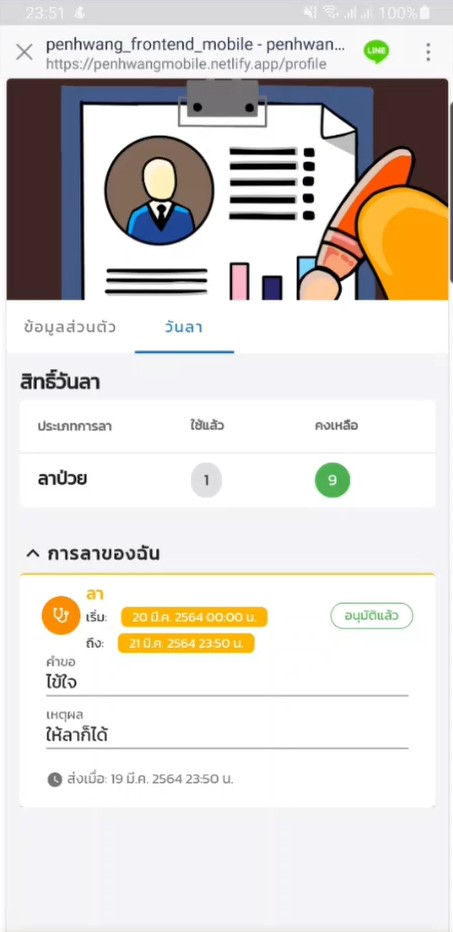
\includegraphics[width=4cm,keepaspectratio]{./images/line_leave_history.jpg}
  \end{center}
  \caption[รูปแสดงประวัติและสิทธิ์การลาในโทรศัพท์มือถือ]{รูปแสดงประวัติและสิทธิ์การลาในโทรศัพท์มือถือ} 
  \label{fig:line_leave_history}
\end{figure}

\begin{figure}
  \begin{center}
    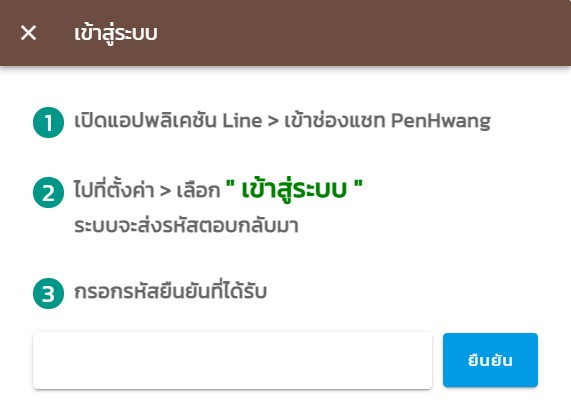
\includegraphics[width=14cm,keepaspectratio]{./images/login.jpg}
  \end{center}
  \caption[รูปแสดงหน้า log-in]{รูปแสดงหน้า log-in} 
  \label{fig:login}
\end{figure}

\begin{figure}
  \begin{center}
    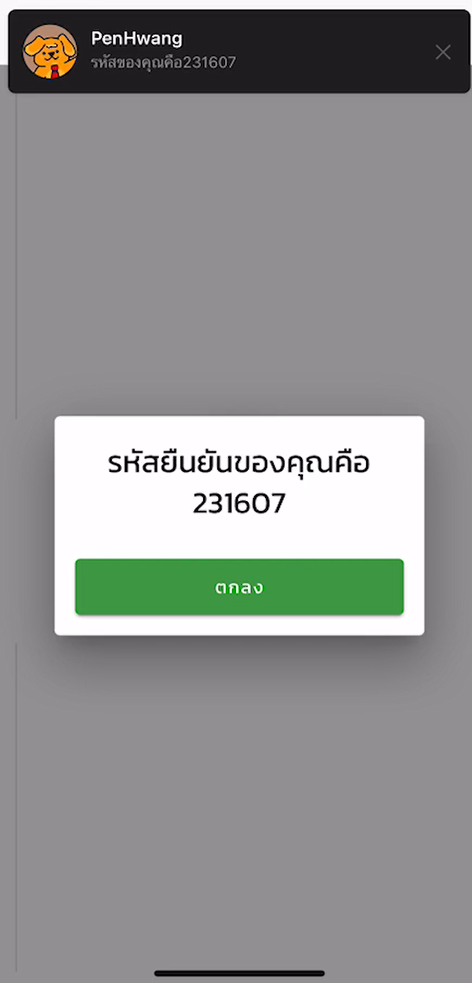
\includegraphics[width=4cm,keepaspectratio]{./images/message_login.png}
  \end{center}
  \caption[รูปแสดงข้อความตอบกลับเมื่อขอ log-in]{รูปแสดงข้อความตอบกลับเมื่อขอ log-in} 
  \label{fig:message_login}
\end{figure}